\documentclass{kththesis}

\usepackage{blindtext} % This is just to get some nonsense text in this template, can be safely removed

\usepackage{csquotes} % Recommended by biblatex
\usepackage{biblatex}
\addbibresource{references.bib} % The file containing our references, in BibTeX format

% Own packages -------------------------------------
\usepackage{multirow}
\usepackage{graphicx}
\usepackage{subcaption}
\usepackage{svg}
\graphicspath{ {images/} }
\usepackage{amsfonts}
\usepackage{amsmath}
\usepackage{siunitx}
\usepackage{soul}
\usepackage[colorinlistoftodos, textsize=tiny]{todonotes}
\usepackage[font=small,labelfont=bf]{caption}  % Make captions smaller

\sisetup{round-mode=figures,round-precision=3}
\sisetup{detect-weight=true}
\usepackage[acronym]{glossaries}
\usepackage{algorithm,algorithmic}% http://ctan.org/pkg/algorithms
\makeglossaries
\newacronym{gan}{GAN}{Generative Adversarial Network}
\newacronym{gans}{GANs}{Generative Adversarial Networks}
\newacronym{vae}{VAE}{Variational Autoencoder}
\newacronym{vaes}{VAEs}{Variational Autoencoders}
\newacronym{mse}{MSE}{Mean Squared Error}
\newacronym{aevb}{AEVB}{Auto Encoding Variational Bayes}
\newacronym{cnn}{CNN}{Convolutional Neural Network}
\newacronym{cnns}{CNNs}{Convolutional Neural Networks}
\newacronym{is}{IS}{Inception Score}
\newacronym{fid}{FID}{Fréchet Inception Distance}
\newacronym{wgan}{WGAN}{Wasserstein GAN}
\newacronym{aegan}{AEGAN}{Autoencoding GAN}
\newacronym{roi}{ROI}{Region Of Interest}
\newacronym{vaegan}{VAEGAN}{Variational Autoencoder + Generative Adversarial Network}
% --------------------------------------------------
% Own commands ---------

\newcommand{\todocomment}[1]{\todo[color=green!40]{#1}}
\newcommand{\todoproofread}[1]{\todo[color=red!40]{#1}}
\newcommand{\ve}[1]{\mathbf{#1}}
\newcommand{\dataset}{\mathcal{S}}
\newcommand{\latentspace}{\mathcal{Z}}
\newcommand{\dataspace}{\mathcal{X}}
\newcommand{\eqdist}{\stackrel{\text{d}}{=}}
% ----------------------

\title{Augmenting High Dimensional Data with Deep Generative Models}
\alttitle{Syntetisk Datagenerering med Djupa Neurala Nätverk för Träning och Evaluering av Pupilregressor}
\author{Mårten Nilsson}
\email{marten3@kth.se}
\supervisor{Josephine Sullivan}
\examiner{Hedvig Kjellström}
\programme{Master in Machine Learning}
\school{School of Computer Science and Communication}
\date{\today}


\begin{document}

% Frontmatter includes the titlepage, abstracts and table-of-contents
\frontmatter

\titlepage

\begin{abstract}
Data augmentation is a techinque that can be performed in various ways to improve the training of discriminative models. The recent developments in deep generative models offer new unexplored ways of augmenting existing data sets. In this thesis, a framework for augmenting annotated data sets with deep generative models is proposed together with a method for quantitatively evaluating the quality of the generated data sets. Using this framework, two data sets for pupil localization is generated with different generative models, including both well-established models and a unique model proposed for this purpose. The unique model was shown both qualitatively and quantitatively to generate the best data sets. A set of smaller experiments on standard data sets also revealed cases where this generative model could improve the performance of an existing discriminative model. The results indicate that generative models can be used to augment or replace existing data sets when training discriminative models.
  %\blindtext
\end{abstract}


\begin{otherlanguage}{swedish}
  \begin{abstract}
    Träutensilierna i ett tryckeri äro ingalunda en oviktig faktor,
    för trevnadens, ordningens och ekonomiens upprätthållande, och
    dock är det icke sällan som sorgliga erfarenheter göras på grund
    af det oförstånd med hvilket kaster, formbräden och regaler
    tillverkas och försäljas Kaster som äro dåligt hopkomna och af
    otillräckligt.
  \end{abstract}
\end{otherlanguage}

\section*{Acknowledgements}
Josephine Sullivan, Hedvig Kjellström, Alexander Davies, Family and Friends etc. 

\tableofcontents


% Mainmatter is where the actual contents of the thesis goes
\mainmatter

% Here's my thesis ---------------------------------------------------------------------------------------

\chapter{Introduction}
%Motivation: Data compresion, can express data sets with smaller space requirements. Improved consistency (better annotations). Semi-supervised learning. Implicit semi-supervised learning.
Establish the context and importance of the topic in this text.

\section{Motivation for synthetic data generation}

\section{Problem statement}

\section{Scope and objectives}

\section{Thesis overview}
Chapter 2 provides and overview of \acrlong{gans} and related methods. The notation used throughout the thesis is establised in section 2.1. In Chapter 3, the method is presented etc...

\subsection{Semi-supervised learning}

\subsection{Data compression}




\chapter{Background}
This chapter begins by establishing the notation and the concepts that are encountered in this chapter. Thereafter a brief overview of generative models is provided. This is followed by an in-depth descriptions of the families of generative modells considered in this project. Finally the concept of semi-supervised learning is introduced.

\section{Concepts and Terminology}
%This chapter deals with high dimensional spaces (written in mathcal, $\mathcal{Z}$), stochastic variables (written in uppercase $Z$), sets (alsa mathcal), vectors (written as plain variables $z$) and probability distributions (reserving the letter $p$ for this, using indexes to distinguish different distributions).
This chapter deals with high dimensional spaces, stochastic variables, sets, vectors and probability distributions. Spaces and sets are written in mathcal ($\mathcal{Z}$), stochastic variables are written as uppercase letters ($Z$), vectors are written as lower case letters ($z$) and the letter $p$ is reserved for probabilities and probability distributions.

\section{Generative models}
\begin{figure}[t]
    \centering
    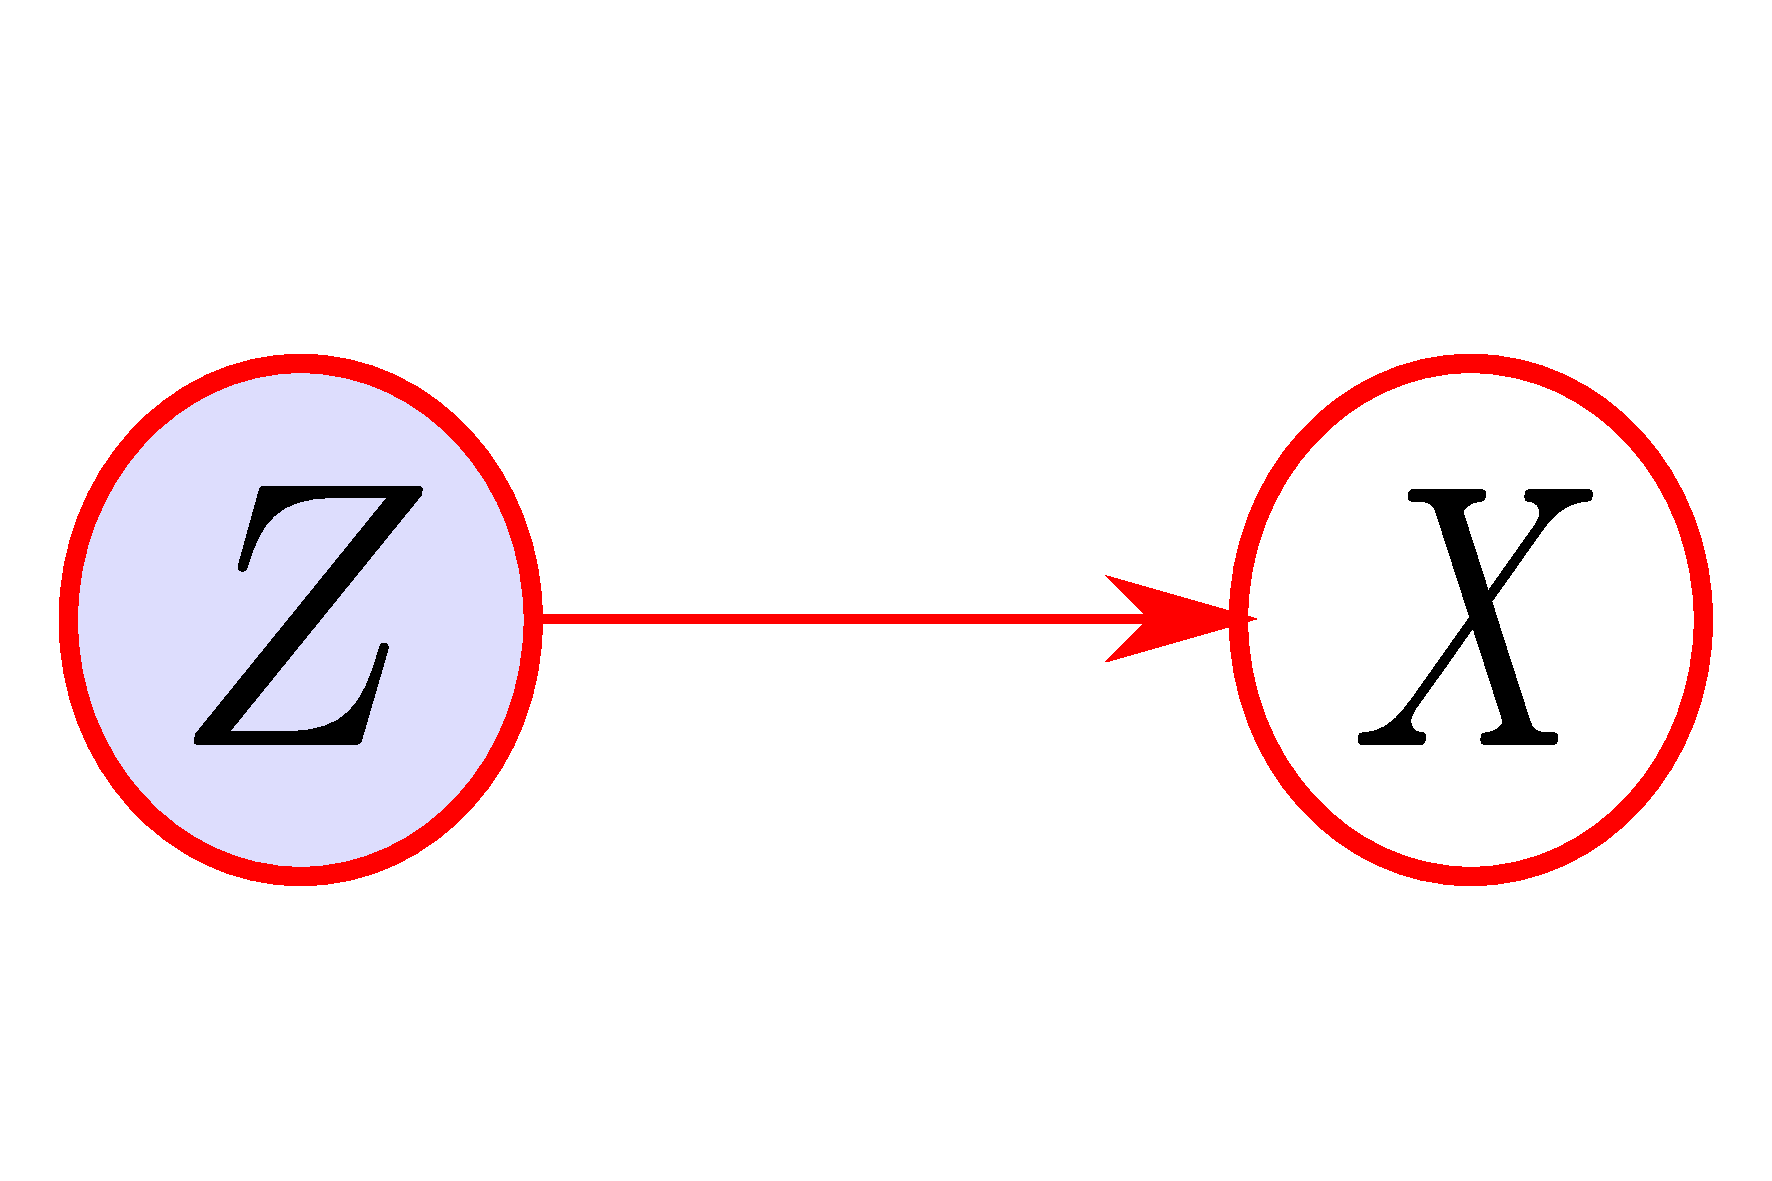
\includegraphics[width=0.5\textwidth]{graphicalModel.pdf}
    \caption{The directed graphical model representing the dependency between the latent variable $Z$ and the data variable $X$ in \acrshort{gans}. This is the same dependency structure as in GMMs and \acrshort{vaes}.}
    \label{fig:GANgraph}
\end{figure}
In this thesis, the term generative model refers to models that explicitly or implicitly represent the data distribution thereby allowing sampling from the modelled distribution. This is different from discriminative models which only model information that can be extracted from the data. 

<<<<<<< HEAD
This thesis focuses on parametric generative models which gan be formulated as instances of probabilistic graphical models \parencite{christopher2016pattern}. Examples of these include Gaussian Mixture Models (GMMs), Hidden Markov models (HMMs), \acrfull{gans} and \acrfull{vaes}. The attention of this work is directed towards models that are applicable on large, high-dimensional and complex data sets. The known models with these properties are  \acrshort{gans} and \acrshort{vaes}. Both of these assume a dependency between a latent variable $Z$ and an observed variable $X$ according to figure \ref{fig:GANgraph}. The rest of this chapter provides a more in-depth description of these models. 
=======
This thesis focuses on parametric generative models which can be formulated as instances of probabilistic graphical models \parencite{christopher2016pattern}. Examples of these include Gaussian Mixture Models, Hidden Markov models, \acrfull{gans} and \acrfull{vaes}. The attention of this work is directed towards models that are computationally tractable on large, high-dimensional and complex data sets. The known models with these properties are  \acrshort{gans} and \acrshort{vaes}. Both of these assume a casual dependency between a latent variable $Z$ and an observed variable $X$ according to figure \ref{fig:GANgraph}. The rest of this chapter provides a more in-depth description of these models. 
>>>>>>> 4886d906f95b333ed286f024e531f582fb58fd74

%Write short state of generative models. Boltzmann machine, explicit models, variational autoencoders etc...

\section{\acrlong{gans}}

\begin{figure}
    \centering
    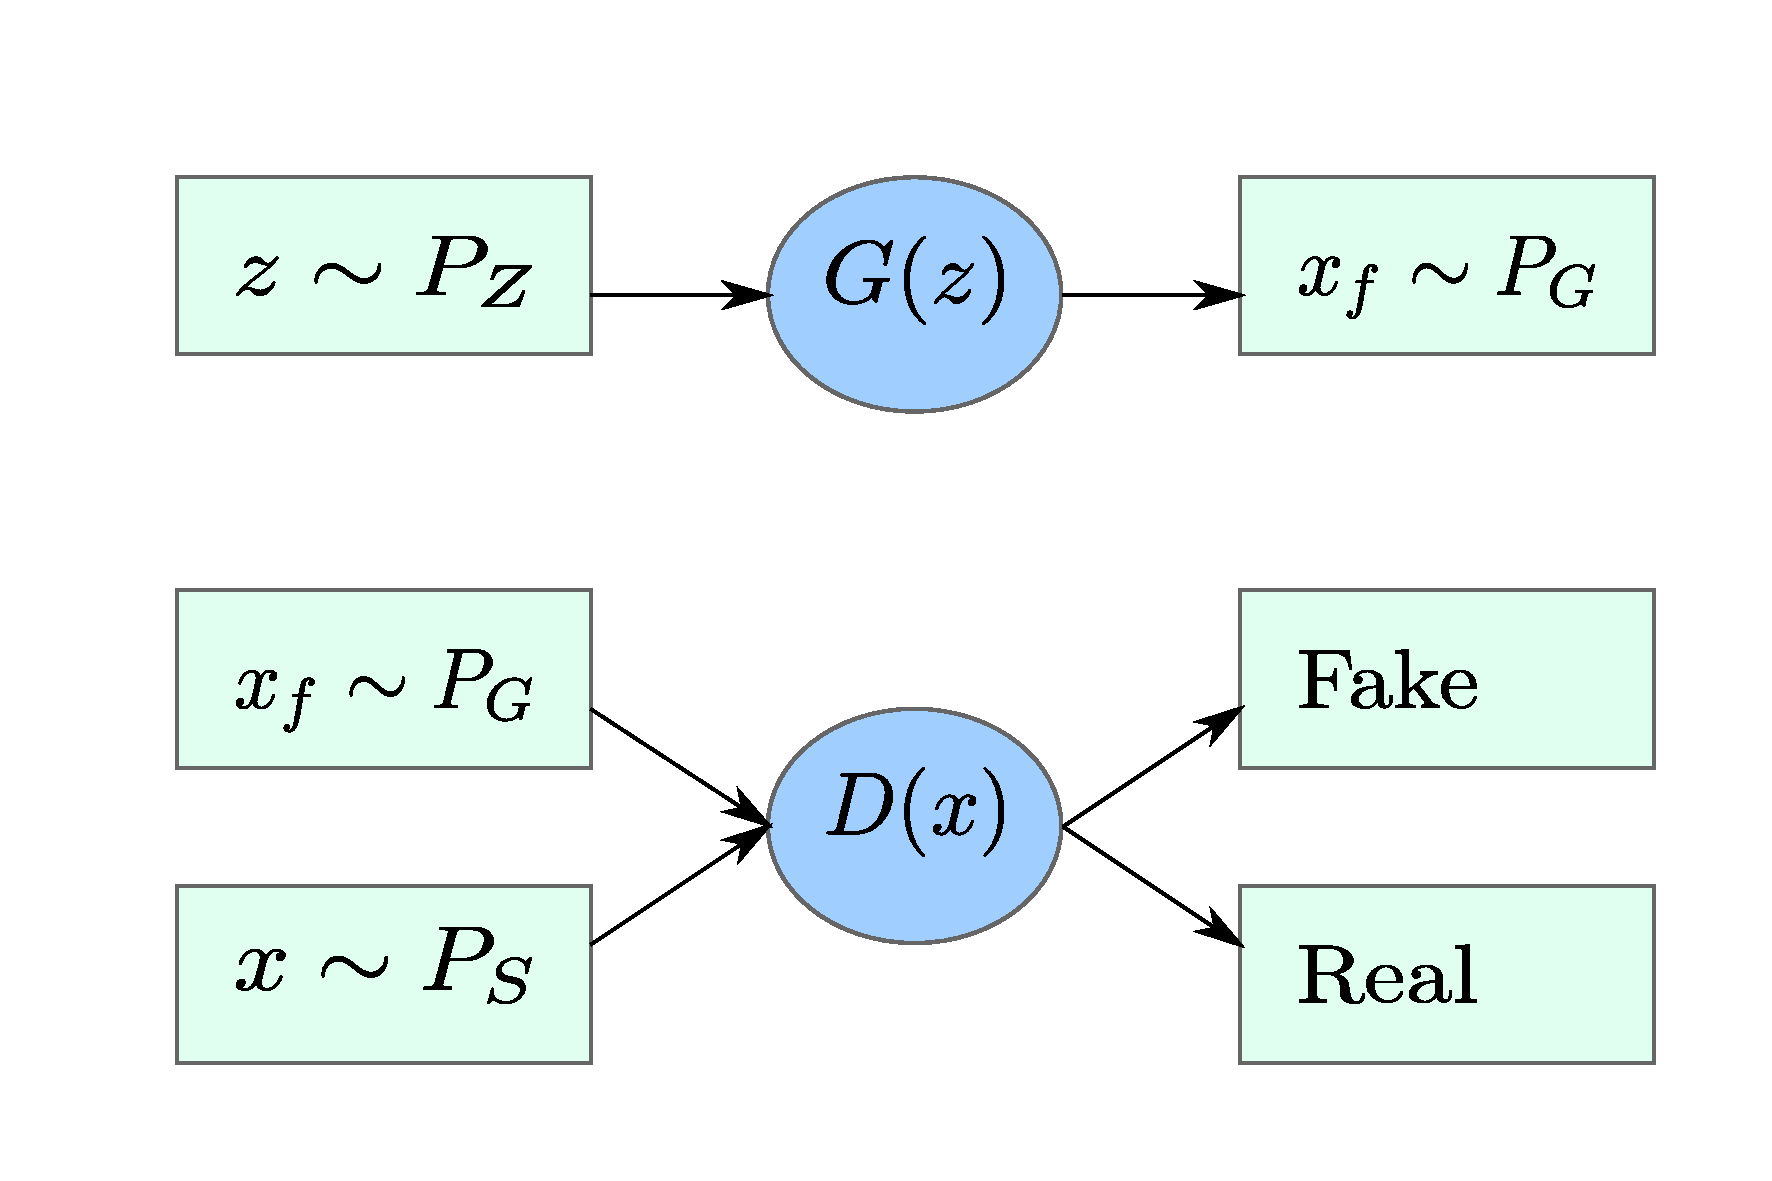
\includegraphics[width=\textwidth]{GANcomponents.pdf}
    \caption{The main components of \acrshort{gans}}
    \label{fig:GAN}
\end{figure}

\acrfull{gans} are a family of generative models proposed by \textcite{goodfellow2014generative}. The framework for training \acrshort{gans} consists of a data set $\dataset$ with elements in a domain $\dataspace$, a latent space $\latentspace$ and two neural networks, a generator $G(z)$ and a discriminator $D(x)$ (figure \ref{fig:GAN}). The generator maps elements of $\latentspace$ to $\dataspace$, $G: \latentspace \rightarrow \dataspace$. The discriminator is a binary classifier $D: \dataspace \rightarrow [0, 1]$. 

The objective of the discriminator is to classify elements in $\dataspace$ as either members or not members of $\dataset$. Members of $\dataset$ are usually referred to as real samples since they are part of the data set, and non-members are referred to as fake samples. The objective of the generator is to fool the discriminator by mapping elements in $\latentspace$ to the subspace of $\dataspace$ that is classified as real. 

The generator can be viewed as representing a probability distribution $p_G$ on $\dataspace$. By introducing a latent random variable $Z$ with the probability distribution $p_Z$ on $\latentspace$, the generator probability distribution can be expressed as $p_G(x) = p_Z(G^{-1}(x))$. 

In practice $G^{-1}$ is intractable to compute, whereby explicit probabilities are seldom acquired through \acrshort{gans}. However, this formulation allows sampling from the learned distribution as $G(z), z \sim p_Z$ is straightforward to compute. 

The goal of training \acrshort{gans} is to learn a probability distribution over the data. By viewing the elements of $\dataset$ as outcomes of a random variable $S$ with probability distribution $p_S$ the goal of the generator is to approximate this distribution with $p_G$, and the goal of the discriminator is to discriminate between these distributions. Using this formulation the objective of the \acrshort{gan} training can be formulated as a minimax game 
\begin{equation}
    \min_G \max_D -J^{D}(G, D)
\end{equation}
where $J^D(G, D)$ is the discriminator cost function from \parencite{goodfellow2016nips},
\begin{equation}
    J^D(G, D) = -\frac{1}{2}\mathbb{E}_{x \sim p_S, z \sim p_Z}\left[\log(D(x)) + \log(1 - D(G(z))) \right].
    \label{eq:GANcost}
\end{equation}
%\begin{equation}
%    \mathcal{L}(x_1, x_2) = -\log(D(x)) + \log(D(x_2)), \quad \begin{cases} x \in X \\ z \in \latentspace \end{cases}.
%\end{equation}
Since both the generator and discriminator are differentiable functions, (\ref{eq:GANcost}) can be optimized using standard gradient based optimization schemes such as RMSprop \parencite{tieleman2012lecture} or Adam \parencite{kingma2014adam}. Typically the networks are updated in an alternating fashion where the parameters of one of the networks are frozen while updating the other network. The expectectations in (\ref{eq:GANcost}) are typically estimated using minibatches as 
\begin{equation}
    \mathbb{E}_{x\sim p(x)}[f(x)] \approx \frac{1}{m}\sum_{i=1}^mf(x_i)
\end{equation}
where $x_i$ is sampled from $p(x)$. This process is described in an algorithmic fashion in Algorithm \ref{alg:GANbase}.


\begin{algorithm}
    \caption{Training scheme for \acrlong{gans} using minibatch stochastic gradient based optimization and $n_D$ discriminator updates per generator update. $\theta_D$ denotes the discriminator parameters and $\theta_G$ denotes the generator parameters.}
    \label{alg:GANbase}
    \begin{algorithmic}[1]
        \FOR{number of iterations}
        \FOR{$n_D$ steps do}
        \STATE sample minibatch of fake data $\{x_{f1}, ..., x_{fm}\} \sim p_G(x)$.
        \STATE sample minibatch of real data $\{x_{1}, ..., x_{m}\} \sim p_S(x)$.
        \STATE update discriminator parameters with the estimated gradient of the cost function
        \begin{equation}
            \nonumber
            \nabla_{\theta_D} \left( -\frac{1}{m}\sum_{i=1}^m\log(D(x_i)) + \log(1-D(x_{fi})) \right).
        \end{equation}
        \ENDFOR
        \STATE sample minibatch of fake images $\{x_{f1}, ..., x_{fm}\} \sim p_G(x)$.
        \STATE update generator parameters with the estimated gradient of the negative cost function
        \begin{equation}
            \nonumber
            \nabla_{\theta_G} \left( - \frac{1}{m}\sum_{i=1}^m\log(1-D(x_{fi})) \right).
        \end{equation}
        \ENDFOR
    \end{algorithmic}
\end{algorithm}


\subsection{Theoretical properties of \acrshort{gans}}
In the original paper (\textcite{goodfellow2014generative}) a couple of theoretical properties of \acrshort{gans} are formulated and proved. These proofs assume that both the generator and discriminator have infinite capacity.

Firstly it is proven that given a fixed generator $G$ the optimal discriminator is 
\begin{equation}
    D(x) = \frac{p_S(X=x)}{p_S(X=x) + p_G(X=x)}.
\end{equation}
A straightforward implication of this is that when $G$ is optimal, the optimal $D$ always output $0.5$ for all real and fake data points. In other words
\begin{equation}
    p_G \eqdist p_S \implies D(x) = 0.5 \; \forall x \sim p_G, p_S
\end{equation}
if $D$ and $G$ are optimal. Secondly, it is also proved in the original paper that given an optimal discriminator there exists a global maximum of the discriminator cost function and it is reached if and only if $p_G \eqdist p_S$. Finally convergence of the training algorithm (Algorithm \ref{alg:GANbase}) is also proven.

This means that one can observe convergence when training \acrshort{gans} by observing the discriminator output. When it saturates at $0.5$ for all generator samples and real samples the algorithm has converged. In practice it is difficult to get to this point with complex sets of high-dimensional data.

\subsection{Practical issues}
The theoretical properties indicate that \acrshort{gans} are a sensible method for implicitly learning probability distributions. However when implementing these models in practice some issues emerge from using models of finite capacity. 

The two-player minimax formulation of the game results in a notoriously difficult training scenario. The update of one player may undo progress of the other player instead of moving towards Nash Equilibrium. Therefore regular gradient descent is not guaranteed to converge but can just as easily get stuck in a stale orbit \textcite{salimans2016improved}. It is also common that the generator learns to represent a subset of the original data realistically while ignoring the vast majority of the data points, thereby collapsing to a specific "mode" of the data. This phenomenon is known as mode collapse.

Another issue encountered when implementing \acrshort{gans} in practice emerges from the limitations of representing a continous distribution with a finite data set. Even though the theoretical results guarantee $p_G$ converges to $p_S$, $p_S$ is not uniquely determined. In fact, $p_S$ is represented by sampling from a uniform discrete distribution over the data set $\dataset$. Therefore the optimal generator would theoretically collapse to this discrete distribution. This results in a generator incapable of generalizing to new data points. On the other hand, should this behaviour be encoutered in practice with limited capacity, the model would still be usable as a compression of the data for applications that only require sampling from the data set. An example for this is using the generator as a proxy for the data set during training or evaluation of another neural network.
 
\subsection{Different types of \acrshort{gans}}
Since the introduction of \acrshort{gans}, several variations and extensions have been proposed to overcome the convergence problems and stability issues of the models. The most relevant variations for this work are outlined in this section.

\subsubsection{Non Saturating \acrshort{gan}} 
An issue with training \acrshort{gans} on the original discriminator cost function (\ref{eq:GANcost}) is that the adversarial term $\log(1-D(G(Z)))$ saturates if the discriminator is too confident. This can prevent the generator from learning in the beginning when the generator output are quite dissimilar to the original data. In the original article it is suggested to train the generator to minimize $-\log(D(G(Z))$ instead. This cost is sometimes referred to as the non saturating const function.

The non saturating cost function preserves the fixed point dynamics of the original \acrshort{gan} formulation while at the same time permitting the generator to learn when the discriminator is confident. Due to this property, non saturating \acrshort{gans} are the implementation used for the experiments in the original article.

\subsubsection{DCGAN}
In an attempt to bring the success of \acrfull{cnns} from supervised to unsupervised learning, \textcite{radfordMC152015} presented a set of architectural guidelines for designing \acrshort{gans} for image generation. They showed that their architectural guidelines resulted in improved quality of the generated samples compared to the state of the art at the time. The guidelines they presented are:

\begin{itemize}
    \item Use strided convolutions instead of pooling in discriminator. Upsample with fractional-strided convolutions in generator.
    \item Apply batch normalization \parencite{ioffeS15batchnorm} in both networks.
    \item Avoid fully connected hidden layers in deeper architectures.
    \item Use ReLU as an activation function in generator and LeakyReLU in the discriminator.
\end{itemize}

Subsequent work have shown alternatives towards some of these guidelines. For an example, batch normalization results in an unwanted correlation between the generated samples in a minibatch \parencite{xiang2017effects}, whereby alternative normalizations have been applied to achieve the desired effects \parencite{karras2017progressive, miyato2017spectral}.

\subsubsection{Conditional \acrshort{gan}}
A limitation of the \acrshort{gan} framework is that it does not allow external information such as image annotations to be modeled. A straightforward extension of the original framework is to let the generator model the conditional distribution $p_S(X|Y)$, where $Y$ represents the additional information. This was proposed in the original article, and was later formally introduced and tested on MNIST\footnote{\textcite{lecun2010mnist}} by \textcite{mirza2014conditional}. The conditional distributions are modeled by introducing the additional information as input to both the discriminator and the classifier.


\subsubsection{Auxiliary Classifier GAN}
The Auxiliary Classifier GAN, proposed by \textcite{odena2016conditional}, is another approach of modelling conditional distributions with \acrshort{gans}. As in the normal conditional \acrshort{gan}, the generator recieves an outcome from both the latent variable $Z$ and the conditional variable $Y$ and generates a sample from this information. In this case the conditional variable is assumed to be a class label, but the approach is easily extendible. In contrast to the generator, the discriminator only recieves the generated sample without any class label. Instead, the discriminator simultaneously attempts to discriminate between real and fake images, as well as producing label class probabilities.

<<<<<<< HEAD
In this framework, the generator is trained to simultaneously produce data points that yields confident correct class predictions at the same time as they are indistinguishable from the correct data points. This approach have been shown to generate images with state of the art \acrlong{is} values at the time \parencite{odena2016conditional}.
=======
In this framework, the generator is trained to simultaneously produce data points that yields confident correct class predictions at the same time as they are indistinguishable from the correct data points. This approach has been shown to generate images with state of the art \acrshort{is} values at the time \parencite{odena2016conditional}.
>>>>>>> 4886d906f95b333ed286f024e531f582fb58fd74

%A problem with this constellation is that the generator is biased towards learning to generate images that can easily be classified. This means that the optimal discriminator doesn't necessarily provide $p_G \eqdist p_S$. It has been shown that the distribution bias introduced by this model causes the generator to completely avoid generating ones with serifs when trained on MNIST despite the high frequency of serifed ones in the data set \textcite{shuac2017acganisbad}.

%\subsubsection{BiGAN}
%Can utilize the latent space.

\subsubsection{Wasserstein GAN}
A popular alternative to the original \acrshort{gan} is the Wasserstein \acrshort{gan}. It was proposed n 2017 by \textcite{arjovsky2017wasserstein}. The distinguishing feature of the Wasserstein \acrshort{gan} is that instead of minimizing the Jensen-Shannon divergence it minimizes the Wasserstein-1, or Earth-Mover EM, distance 
\begin{equation}
    W(p_S, p_G) = \inf_{\gamma \Pi (p_S, p_G)} \mathbb{E}_{(x, y) \sim \gamma} \left[|x-y|\right],
\end{equation}
where $\Pi(p_s, p_g)$ is the set of all joint distributions with $p_S$ and $p_G$ as marginals. \textcite{arjovsky2017wasserstein} illustrated that this is equivalent to minimizing the cost function
\begin{equation}
    W^{(D)}(D, G) = \mathbb{E}_{x\sim p_S}[D(x)] - \mathbb{E}_{z \sim p_Z}[D(G(z))],
\end{equation}
under the constraint that $D$ is Lipschitz smooth. \textcite{arjovsky2017wasserstein} enforced Lipschitz smoothnes by clipping the weights of the discriminator. In subsequent works more sophisticated methods have been proposed such as gradient penalty \parencite{gulrajani2017improved}, weight normalization \parencite{NIPS2016\_6114} and spectral normalization \parencite{miyato2017spectral}.

%\subsubsection{BEGAN}
%\subsubsection{DRAGAN}
\subsubsection{Progressive GAN}
\textcite{karras2017progressive} proposed a novel training methodology for \acrshort{gans} to address the stability and variability issues with these models when trained to generate images. The proposed methodology regards the network architectures during training and can be combined with many of the other \acrshort{gan} variants seamlessly. Instead of training a fixed-size discriminator and generator it is proposed to progressively grow their size during training by gradually increase the resolution of the training data. Since training on higher resolution images is much more difficult that on low resolution images, this method conceptually acts as iteratively reusing a simpler network as a sensible initialization for the next higher-resolution network. It can also be veiwed as a multi-step transfer learning process. This approach demonstrated high-quality diverse fake samples on a 1028x1028 version of the CELEBA (write this in better font) dataset. 

Besides the progressive growing of \acrshort{gans}, \textcite{karras2017progressive} also suggest two improvements that can be applied on other variants as well. They propose weight equalization to address the issue of training deep networks with weights that have different dynamic range. They propose using a pixelwise normalization of the feature maps instead of batch normalization to prevent escalation of signal magnitudes between the networks.

\subsection{Evaluation measures}
The goal of \acrshort{gans} is to model a target distribution and they are often trained on high-dimensional complex data sets. Due to the nature of this setup and the observation that explicit probabilities are unobtainable for both the true data distribution and the modeled distribution, these models are difficult to evaluate. Two popular quantitative measures for evaluating the performance of \acrshort{gans} are the \acrfull{is} \parencite{salimans2016improved} and the \acrfull{fid} scores \parencite{heuselRUNKH2017FID}.

The \acrlong{is} metric was defined as an alternative to having human annotators asses the quality of visual samples. It is defined as 
\begin{equation}
    \exp (\mathbb{E}(D_{KL}(p(Y|X) || p(Y))))
\end{equation}
where $p(Y|X)$ is the class conditional probability distribution obtained through a pretrained inception network and $p(Y)$ is obtained through marginalization. 

The \acrlong{fid} metric is a proposed improvement over the \acrlong{is}. Unlike the \acrlong{is}, the \acrlong{fid} metric measures the distance between the learned data distribution and the true distribution. It does so by computing the Frechét distance (Wasserstein-2 distance) between inception encodings of the true data distribution and the fake data distribution.

<<<<<<< HEAD
These measures have been shown to correspond to increased quality and diversity of generated samples but do still inherently suffer from the limitations imposed by the abscence of explicit probability distributions. For an example, \textcite{shuac2017acganisbad} showed that the ACGAN generator is biased towards learning to generate images that can easily be classified. This means that the training doesn't necessarily converge towards $p_G \eqdist p_S$. This bias was both theoretically established and experimentally verified by training an ACGAN on MNIST and observing that generator completely avoid generating ones with serifs despite the high frequency of serifed ones in the data set. This skew in data distribution is not quantitatively apparent as the model was shown to still result in high \acrshort{is} values. In fact the ACGAN model obtained higher scores than the original data set. Similar examples for the \acrshort{fid} have not been discovered during the course of this project. 
=======
These measures have been shown to correspond to increased quality and diversity of generated samples but do still inherently suffer from the limitations imposed by the abscence of explicit probability distributions. As an example, \textcite{shuac2017acganisbad} showed that the ACGAN generator is biased towards learning to generate images that can easily be classified. This means that the training doesn't necessarily converge towards $p_G \eqdist p_S$. This bias was both theoretically established and experimentally verified by training an ACGAN on MNIST and observing that the generator completely avoid generating ones with serifs despite the high frequency of serifed ones in the data set. This skew in the data distribution is not quantitatively apparent as the model was shown to still result in high \acrshort{is} values. In fact the ACGAN model obtained higher scores than the original data set.
>>>>>>> 4886d906f95b333ed286f024e531f582fb58fd74

In specific applications, the quality of the generated samples can be evaluated indirectly based on the application of the data. \textcite{shrivastava2016learning} used this approach to compare the quality of a generated data set against the real data alone for gaze estimation. This approach does not guarantee correspondence between visually pleasing samples and generated samples and does not allow the results to be compared with similar \acrshort{gans} in a different domain. However it is appealing in the sense that it brings the quantitative evaluation of the models closer to the targeted application. 

\subsection{Evaluation issues}
Besides the difficulties in finding quantitative evaluation measures, \acrshort{gans} are vere sensitive to hyperparameter setting and it is difficult to assess if improved results are caused by better hyperparameters or improved methods. This was demonstrated in a recent work by \textcite{lucic2017gans}, where a large scale evaluation of some of the state-of-the-art variants was performed. It was observed that similar results could be obtained for all the models as a result of enough random restarts and hyperparameter optimization.

In parallel with the empirical comparisons of different \acrshort{gans} theoretical arguments regarding the objective of these models are taking place. \textcite{arjovsky2017towards} introduced the divergence that the NSGAN minimizes, and argues why this causes mode collapse and convergence issues. The view on the training of \acrshort{gans} as minimization of a divergence have subsequently been critizised as overly restrictive, and empirical counterexamples have been presented to challenge this view \textcite{fedus2017many}.


\section{\acrlong{vaes}}
Another popular family of generative models besides \acrshort{gans} are \acrfull{vaes}. \acrlong{vaes} were first introduced by \textcite{kingma2013auto} as a scalable approach for stochastic variational inference. \acrshort{vaes} are trained using the \acrfull{aevb} algorithm proposed in the same article. 

These models consists of an i.i.d. data set $\dataset$ and a continous latent variable $Z$ in a latent space $\latentspace$. The data set is viewed as a set of outcomes of a random variable $S$ as previously. The prior $p(Z)$ and likelihood $p(S|Z)$ are assumed to come from parametric families of distributions and the posterior $p(Z|S)$ is assumed to be intractable and is modeled by some parametric distribution. The parameters of the prior and likelihood distribution are commonly denoted as the generative model parameters $\theta$. The probabilities in the context of these model are commonly denoted as $p_\theta(X)$, $p_\theta(X|Z)$ and $p_\theta(Z|X)$ to explicitly expose the model parameters. Since the posterior $p_\theta(Z|X)$ is assumed intractable it is estimated with a variational approximation, commonly denoted $q_\phi(Z|X)$. From the deep learning perspective, $q_\phi(Z|X)$ is commonly refered to as the \textit{encoder}, and $p_\theta(X|Z)$ is commonly referred to as the \textit{decoder}.

The \acrshort{aevb} algorithm is applied to learn the generative model parameters and infer the optimal variational parameters. It is a type of approximate variational inference and consists of gradient based optimization of an estimatior of the variational lower bound of the marginal likelihood of the data under the current model. In the original article the authors propose the two estimators based on Monte Carlo estimates of expectations:
\begin{equation}
    \label{eq:VAEstimators}
    \begin{aligned}
        \mathcal{L}^A = \frac{1}{L}\sum_{l=1}^L \log p_\theta (X=x^{(i)},Z=z^{(i, l)}) - \log q_\phi (Z=z^{(i, l)} | X=x^{(i)}) ), \\
        \mathcal{L}^B = - D_{KL}(q_\phi (Z | X=x^{(i)}) || p_\theta(Z=z)) + \frac{1}{L}\sum_{l=1}^L \log p_\theta (X=x^{(i)},Z=z^{(i, l)}).
    \end{aligned}
\end{equation}

\begin{algorithm}
    \caption{Training scheme for \acrlong{vaes}}
    \label{alg:VAEbase}
    \begin{algorithmic}[1]
        \FOR{number of iterations}
        \STATE sample minibatch of data points $\{x_{1}, ..., x_{m}\} \sim p_S(x)$.
        \STATE sample minibatch from the latent space $\{z_1, ..., z_m\} \sim p_\theta(z)$.
        \STATE update model parameters with gradients of any of the proposed estimators in equation \ref{eq:VAEstimators}.
        \ENDFOR
    \end{algorithmic}
\end{algorithm}

\acrshort{vaes} can be trained by maximizing either of these estimates using common gradient based methods as described in Algorithm \ref{alg:VAEbase}. An issue with this approach is that the lower bound estimates require sampling from the latent variable, which is a non-differentiable operation. \textcite{kingma2013auto} resolved this issue by introducing a reparametrization trick to enable gradients to flow through the sampling process. This is applied in Algorithm \ref{alg:VAEbase}, but will not be explained in detail in this report for brevity. The illustrations in \parencite{doersch2016tutorial} are an excellent source of intuition why this works.

\subsection{Combining \acrshort{vaes} with \acrshort{gans}}
Both \acrshort{vaes} and \acrshort{gans} implicitly model the data distribution $p_S(x)$ by introducing a latent stochastic variable Z. \acrshort{vaes} model the posterior of the latent variable and learn using the KL divergence on this posterior as well as the reconstruction loss of the data after sampling. \acrshort{gans} on the other hand directly generate samples from the prior of the latent variable and uses the discriminator network as an adversarial loss function on the generated samples. 

The similarity of these approaches allows different methods of combining the benefits of both approaches. The most straightforward approach of training a \acrshort{vae} with an adversarial loss function was performed by \textcite{LarsenSW15autoencodingbeyond}. The resulting model generated sharp realistic-looking samples and allowed meaningful arithmetic to be performed in the latent space.

\section{Semi-supervised learning}
\begin{figure}
    \centering
    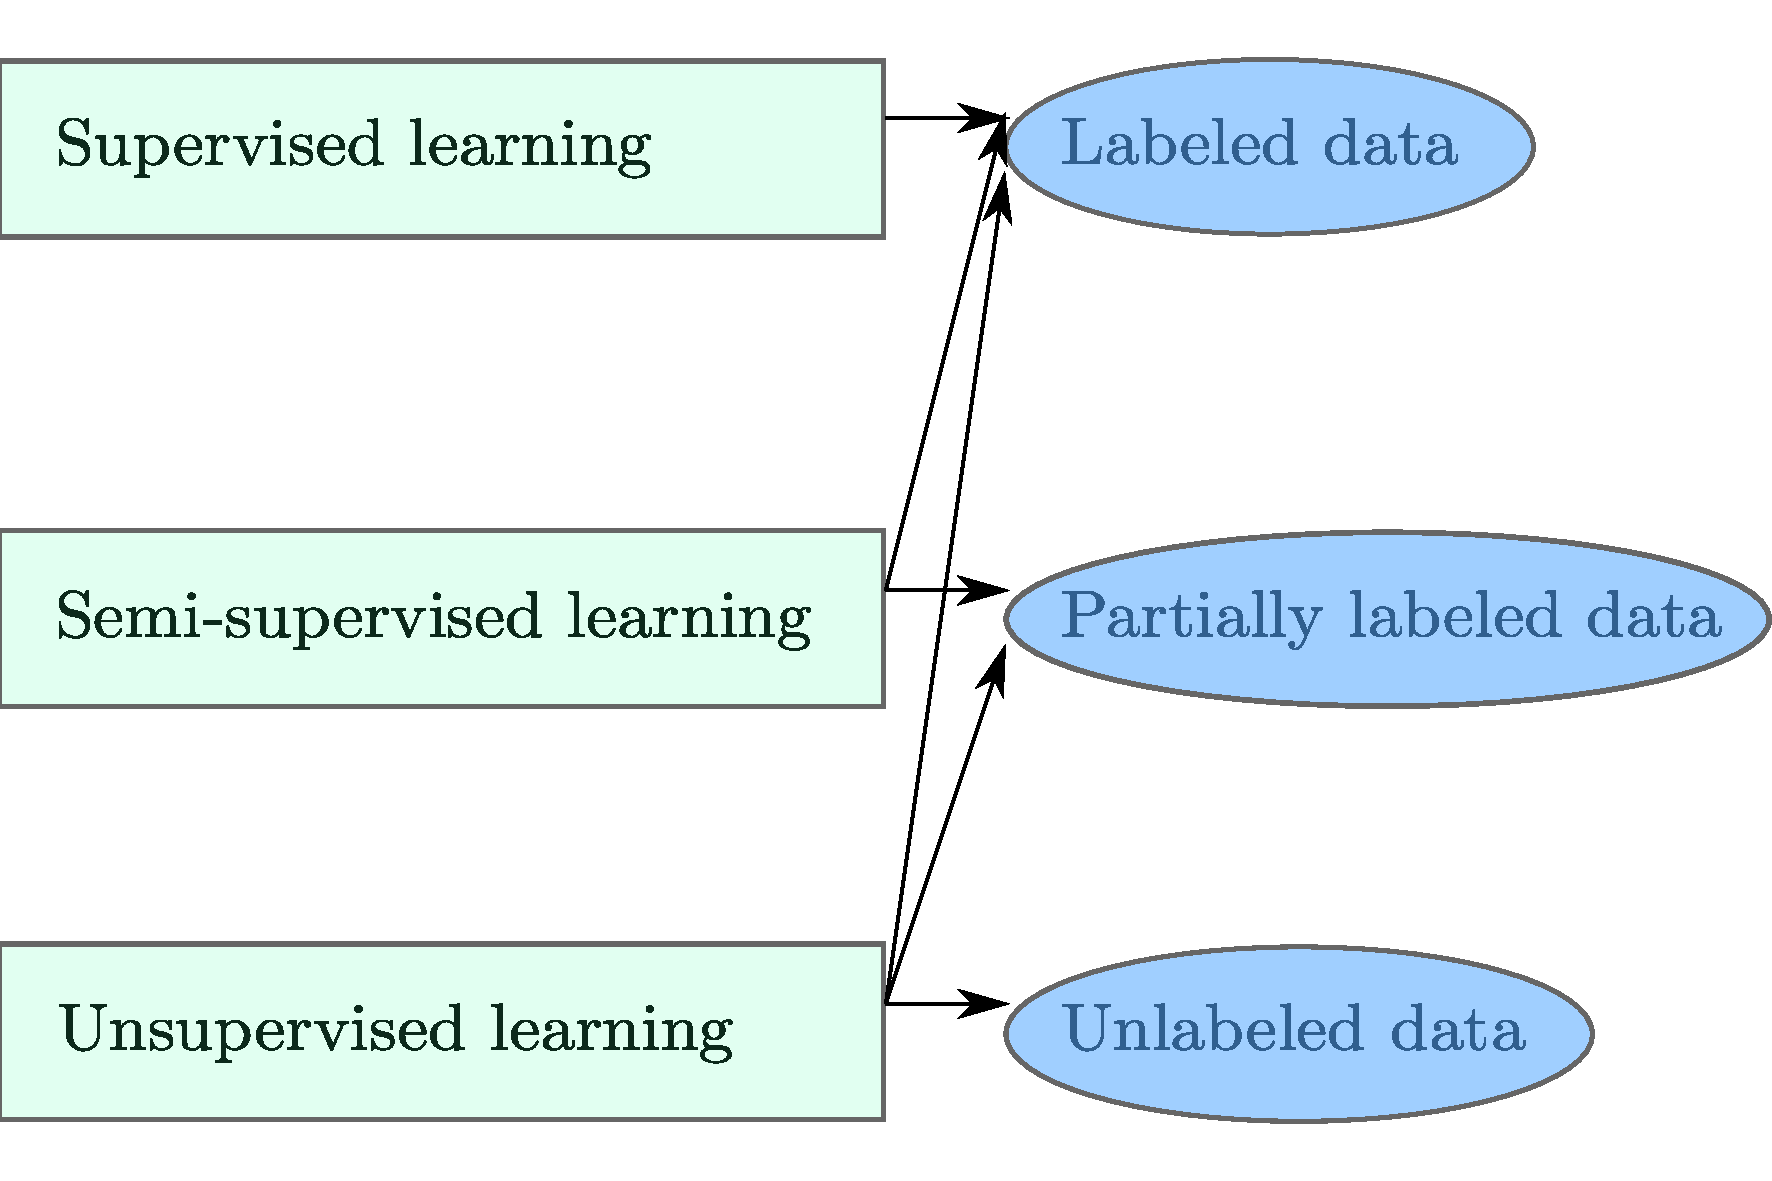
\includegraphics[width=\textwidth]{supersemiun.pdf}
    \caption{Levels of supervision in Machine Learning. Unsuperviesd algorithms are not dependent on labels and can therefore be applied on any type of data, whereas supervised algorithms require fully annotated data sets. Semi-supervised learning emerges as a middle ground between the two approaches.}
    \label{fig:supersemiun}
\end{figure}
Supervised learning can be seen as the problem of learning from data that is structured in pairs of patterns ($x$) and labels ($y$). The data set can consequently be represented as $S = {(x_1, y_1), ..., (x_n, y_n)}$. The task is then to predict the labels given the patterns. This transitions to semi-supervised learning when the training data does not necessarily contain labels for each pattern. The relations between the classes of supervision is illustrated in figure \ref{fig:supersemiun}. 

Methods for semi-supervised learning have shown success in improving the accuracy of supervised methods in settings where labeled data are limited \parencite{Zhou2012}. Generative models are well suited for semi-supervised learning, and several methods building on deep generative models have been proposed \parencite{kingma2014semi, salimans2016improved, springenberg2015unsupervised, wuliu2017selftrainsemisup, li2017triple}.

<<<<<<< HEAD
A common method for semi-supervised learning is self training. Self training is based on computing estimates of the missing labels which subsequently are reused for training the network. An interesting instance of self training when considering \acrshort{gans} is the triple \acrshort{gan} \parencite{li2017triple}. The triple \acrshort{gan} is a conditional \acrshort{gan} where the generator network is accompanied by a classifier network, which predicts the labels given the data. This network is also trained with and adversarial loss, at the same time as it is used to generate annotations for the generator. This constellation allows the networks to be trained on large amounts of unlabeled data when the classifier converges faster than the generator, which normally is the case.

The triple \acrshort{gan} is closesly related to the $\Delta$-\acrshort{gan} \parencite{triangleNIPS20177109} which also allows semi-supervised learning. The semi-supervised learning proposed for the $\Delta$-\acrshort{gan} is unlike the triple \acrshort{gan} not based on self training. Instead the objective function can be decomposed into a conditional part and a bidirectional part which can account for labeled and unlabeled data separately.
=======
A common method for semi-supervised learning is self training. Self training is based on computing estimates of the missing labels which subsequently are reused for training the network. An interesting instance of self training when considering \acrshort{gans} is the triple \acrshort{gan}, which is a conditional \acrshort{gan} where the generator network is accompanied by a classifier network, which predicts the labels given the data. This network is also trained with an adversarial loss, at the same time as it is used to generate annotations for the generator. This constellation allows the networks to be trained on large amounts of unlabeled data when the classifier converges faster than the generator, which normally is the case.
>>>>>>> 4886d906f95b333ed286f024e531f582fb58fd74

%\section{Image-to-Image Models}

%\section{Common architectures}

%\section{Normalization techniques}

%\section{Related work}
%Hmm, värt att nämna? 








\chapter{Methods}
%Here is the method used to examine the question
In this chapter, the methods employed to answer the proposed question are presented. This chapter begins by establishing the task, data sets and data processing utilized in this project. Thereafter, the experimental setup is described and relevant neural network architectures are outlined. Finally, the approaches for training the generative models are presented. Three approaches of this kind have been employed in this project: standard \acrfull{vaes}, progressive \acrfull{gans} and Autoencoding \acrfull{gans}. They are presented in their respective section. 

The level of detail presented here should suffice for re-implementing the algorithms and reproduce the experiments of this project. There certainly exists questions which need more details to answer than what can possibly be captured in a report like this. For further details, the original implementation is available online\footnote{The code is availabel at: \url{www.github.com/netrome/DeepGeneration}}.

\section{Pupil Localization}
To investigate the extent to which deep generative models can act as a drop-in replacement for real data sets, a case study of pupil localization was performed. Pupil Localization is an instance of the problem of object localization. The objective is to localize the pupil in an image of an eye. In normal cases, pupil localization is not achieved with deep neural networks. There already exist more computationally efficient methods for this task, such as the method proposed in \parencite{markuvs2014eye}. On the other hand, deep neural networks for semantic segmentation are capable of predicting high quality segmentation maps on diverse complicated data sets \parencite{ChenPK0Y16semantic} and should therefore perform extraordinary well on the relatively simple task of pupil localization.

By comparing pupil localization performance when the localizer is trained on either data from a deep generative model or data from the original data set and tested on data from either of the domains, the usability of the generated data for model training or evaluation can be assessed. This becomes especially interesting in the case of training on generated data and testing on the original data. Assuming that the localizer learns the optimal mapping for the data domain it is trained on, the performance of this localizer can then be used as a measure of the quality and usability of the generated data. 

The benefit of this approach is that the relative magnitutes of the errors obtained when training on one data set and testing on another indicate the difficulties of adapting models between these domains. This does not only give a binary answer to the original question of this project but also shows how close to succeeding the tested methods are in learning the data distribution. %\todocomment{Good summary of the point}

%The benefit of this approach is that the cross-data localization error can easily be compared to the intra-data localization error. The relative magnitutes of these losses indicate the difficulties of adapting models between the domains. This enables not only giving a binary answer to the original question of this project but showing how close to succeeding the tested methods are in learning the data distribution.

\section{Synthetic Data}
The initial experiments in this project are performed on synthetic data obtained through rendering of a 3D head model in a data generation framework. This framework is based on the work of \textcite{swirski2014rendering} and utilizes the same head rig. Two data sets with resolution 256x256 were generated, a training set consisting of 3000 images and a test set of 300 images. For reproducibility, these data sets will become publicly available at the time of publication.

The synthetic data sets are fully annotated with automatically generated ground truth labels. The relevant labels for the experiments are converted to heatmaps when loaded for training and evaluation as in most cases of semantic segmentation \parencite{guo2017review}. These heatmaps are thereafter concatenated with the real images, forming feature maps with the dimensions: 2x320x320. By viewing the annotations as a part of the data, unsupervised models that learn the data distribution implicitly learn the relationships between the annotations and the images.

\section{Real World Data}
A propiretary data set was used to further evaluate the methods. The data set consits of 9605 different manually annotated recordings of human subjects looking at a screen, split into a training set of 1000 recordings and a test set of 8605 recordings. Each recording consists of a set of ROI \todoproofread{add ROI to your accronym package} images of the eye region of the subjects. 

To adapt this data to the Pupil Regression framework, the images were cropped to 256x256 patches around the eyes. The cropping was random to ensure that the pupil \st{is} \todoproofread{was} not always centered in the image, which otherwise \st{could} \todoproofread{would} cause the networks to learn undesired patterns such as always producing a trivial prediction in the center of the image. \todoproofread{Mixing tenses in this sentence}

During data sampling, the probabilites of the individual images were weighted in such a way that the separate recordings were equally probable to appear. This prevents recordings with more images to be \st{over-representative} \todoproofread{over represented} during training, which otherwise could cause the models to \st{over-adjust} become \todoproofread{skewed} to the conditions of these recordings.

\section{Network architectures}
The deep generative models as well as the Pupil Localizer are based on deep convolutional neural networks. There are four different types of networks that are utilized in the different models in this work: Generators, discriminators, encoders and transformers. These types describe the transformation \todoproofread{s} the networks represent.

The default generator architecture is outlined in table \ref{tab:generator}. The default discriminator architecture is outlined in table \ref{tab:discriminator}. The main structure of these networks follows the architectures used by \textcite{karras2017progressive}, however the feature maps are smaller in this project and instead of using non-parametric upsampling followed by an extra convolution \todoproofread{,} the upsampling is performed with fractionally strided convolutions. These changes are motivated by the limited time-frame of this project as they enable faster training of the networks. Furthermore \todoproofread{,} the data sets of this project are believed to be of less complexity than those of \textcite{karras2017progressive}, whereby less parameters should be necessary for the networks to caputre the essence of the data sets.

The encoder follows the structure of the discriminator but does not use minibatch discrimination, and the output shape is adjusted to the size of the latent space instead of producing a scalar output. 

The transformer is only used for Pupil Localization and is a normal image-to-image network. The structure of the transformer is shown in table \ref{tab:transformer}. The main structure resembles that of \textcite{ronneberger2015u}\st{,} but many details are different. \todocomment{is it worth discussing those differences?}

%...relevant network architectures are described here, together with figures and stuff. Base it around GAN networks, the small differences in the encoders can be explained afterwards.

\begin{table}[t]
    \centering
    \caption{Generator architecture used in the experiments. Feature normalization and leaky ReLUs were applied after each convolution except the last one.}
    \label{tab:generator}
    \begin{tabular}{|lll|}
        \hline
        %\multicolumn{3}{c}{Generator}           \\ 
        Operation          & Output shape     & Stride \\ \hline
        Input              & 128x1x1   & 1      \\
        Conv 4x4           & 128x4x4   & 1      \\
        Conv 3x3           & 128x4x4   & 1      \\ \hline
        Transpose Conv 2x2 & 128x8x8   & 2      \\
        Conv 3x3           & 112x8x8   & 1      \\ \hline
        Transpose Conv 2x2 & 11216x16   & 2      \\
        Conv 3x3           & 96x16x16   & 1      \\ \hline
        Transpose Conv 2x2 & 96x32x32   & 2      \\
        Conv 3x3           & 80x32x32   & 1      \\ \hline
        Transpose Conv 2x2 & 80x64x64   & 2      \\
        Conv 3x3           & 64x64x64   & 1      \\ \hline
        Transpose Conv 2x2 & 64x128x128   & 2      \\
        Conv 3x3           & 32x128x128   & 1      \\ \hline
        Transpose Conv 2x2 & 32x256x256   & 2      \\
        Conv 3x3           & 16x256x256   & 1      \\ \hline
        Conv 1x1           & 2x256x256 & 1        \\ \hline
    \end{tabular}
\end{table}

\begin{table}[t]
    \centering
    \caption{Discriminator architecture, Leaky ReLUs were applied after each convolution except the last one.}
    \label{tab:discriminator}
    \begin{tabular}{|lll|}
        \hline
        %\multicolumn{3}{c}{Discriminator}           \\ 
        Operation          & Output shape     & Stride \\ \hline
        Input              & 2x256x256   & 1   \\
        Conv 1x1           & 16x256x256 & 1    \\ 
        Conv 3x3           & 32x256x256 & 1    \\ 
        Conv 2x2           & 32x128x128 & 2    \\ \hline
        Conv 3x3           & 64x128x128 & 1    \\ 
        Conv 2x2           & 64x64x64 & 2      \\ \hline
        Conv 3x3           & 80x64x64 & 1      \\ 
        Conv 2x2           & 80x32x32 & 2      \\ \hline
        Conv 3x3           & 96x32x32 & 1      \\ 
        Conv 2x2           & 96x16x16 & 2      \\ \hline
        Conv 3x3           & 112x16x16 & 1     \\ 
        Conv 2x2           & 112x8x8 & 2       \\ \hline
        Conv 3x3           & 128x8x8 & 1       \\ 
        Conv 2x2           & 128x4x4 & 2       \\ \hline
        Minibatch stddev
        Conv 3x3           & 128x4x4   & 1     \\
        Conv 4x4           & 128x1x1   & 1     \\ 
        Fully connected    & 1x1 & 1         \\ \hline
    \end{tabular}
\end{table}

\begin{table}[t]
    \centering
    \caption{Transformer architecture used in the experiments. Skip layers were introduced as indicated in the table. Leaky ReLUs were applied after each convolution except the last one. In the prescence of skip connections the addition of the feature maps was performed before the Leaky ReLUs were applied.}
    \label{tab:transformer}
    \begin{tabular}{|lll|}
        \hline
        %\multicolumn{3}{c}{Generator}           \\ 
        Operation           & Output shape  & Stride \\ \hline
        Input               & 1x256x256     & 1     \\
        Conv 1x1 (1)           & 16x256x256    & 1     \\
        Conv 3x3 (2)            & 32x128x128    & 2     \\    
        Conv 3x3 (3)           & 64x64x64    & 2     \\ 
        Conv 3x3 (4)           & 128x32x32    & 2    \\ 
        Conv 3x3 (5)           & 256x16x16    & 2    \\ 
        Conv 3x3 (6)           & 256x8x8     & 2    \\ 
        Conv 3x3            & 256x4x4    & 2    \\ \hline
        Transpose Conv 4x4 + (6)  & 256x8x8    & 2    \\
        Transpose Conv 4x4 + (5) & 256x16x16    & 2    \\
        Transpose Conv 4x4 + (4) & 128x32x32    & 2    \\
        Transpose Conv 4x4 + (3) & 64x64x64    & 2    \\
        Transpose Conv 4x4 + (2) & 32x128x128    & 2    \\
        Transpose Conv 4x4 + (1)  & 16x256x256    & 2    \\
        Conv 1x1            & 1x256x256    & 1     \\ \hline
    \end{tabular}
\end{table}

\section{\acrlong{vaes}}
A \acrlong{vae} was constructed and trained on the synthetic data as a baseline for further experiments. The advantages of using \acrshort{vaes} for data generation in contrast to \acrshort{gans} is that they are easier to train and do\st{es} not suffer from vanishing modes of data.

The \acrlong{vae} was designed using the default generator network as a decoder and the default encoder network with an output shape of 128x2. In this framework, the encoder output is interpreted as the mean values and the standard deviations of a 128-dimensional isotropic gaussian distribution. Using $E$ to denote the encoder function, this can be formulated as $P(Z|X=x) \in \mathcal{N}(\mu, \sigma)$, where $(\mu, \sigma) = E(x)$. Furthermore, the posterior $P(X|Z=z)$ is modelled as a Laplace distribution where the mean value is the generator output as $P(X|Z=z) \in \text{Laplace}(G(z), b)$, where $b$ is taken to be a hyperparameter. From a deep learning perspective this is equivalent to training the $VAE$ with a $L_1$ reconstruction loss. The training objective can then be formulated as 
\begin{equation}
    L_{VAE} = \lambda D_{KL}\left(P(Z|X=x) | \mathcal{N}(0,1)\right) + |\hat{X} - X|_1,
\end{equation}
where $\hat{X}$ is the reconstructed image, and $\lambda$ is a scale parameter that controls the trade-off between the KL term and the reconstruction loss. Scaling the KL loss has the same relative effect between the two loss terms as adjusting the $b$ parameter in the Laplacian distribution, and fixing the weight of the $L_1$ loss instead of the $KL$-loss means \todocomment{is the KL term explained somewhere else?} that a sensible learning rate in this setting should be similar to that of a normal autoencoder. 

\section{\acrlong{wgan}}
The \acrfull{wgan} was adopted as a second baseline to compare against more complex methods. It was chosen because it currently is one of the most prominent \acrshort{gan} variations. Furthermore the progressive \acrshort{gan} of next section is based on the \acrshort{wgan} causing it to be both a natural baseline for the evaluation and a special case of the progressive \acrshort{gan}. 

The \acrshort{wgan} was constructed using the default generator and discriminator. To enforce the discriminator to be Lipschitz 1 \todocomment{What is Lipschitz 1?, do you refere to this in your background chapter? If so then you should add a link to it otherwise the reader would have no idea what the point of this statement is"}, gradient penalty was used as described in \parencite{gulrajani2017improved}.

\section{Progressive \acrshort{gan}}
The most advanced method tested in this project was the progressive \acrshort{gan}, proposed by \textcite{karras2017progressive}. The proposed advantages of this approach over other existing \acrshort{gan} variations is two-fold. Firstly, there is reason to believe that the quality and diversity of the generated samples are improved by the progressive training. Secondly, the training stability is believed to increase. However due to the novelty of the approach and the lack of extensive evaluations of different \acrshort{gans} \todoproofread{,} it is difficult to know for sure if this is the case.

The progressive \acrshort{gan} was adopted because of the proposed training stability that arises from progressivly increasing the complexity of the learned task. It was implemented using the default generator and discriminator. The training was divided in six stages, each stage producing images with four times the resoulution of the previous stage. As in the original article, each stage contained an extra 1x1 convolution to produce 2-channel images. \todocomment{I think a diagram illustrating the progressive GAN training process would be beneficial} The illustrated networks are therefore examples of stage-6 networks. To obtain a stage-5 network one should simply reshape the 1x1 convolutions and remove the two last (non 1x1) convolutions of the generator and the two first (non 1x1) convolutions of the generator.

As in the original article, feature normalization, minibatch discrimination and smooth fade-in of new layers was implemented as closely as possible to the original formulation.

%\subsection{Freeze in new layers}
%\begin{figure}[t]
%    \centering
%    \begin{subfigure}[b]{0.45\textwidth}
%        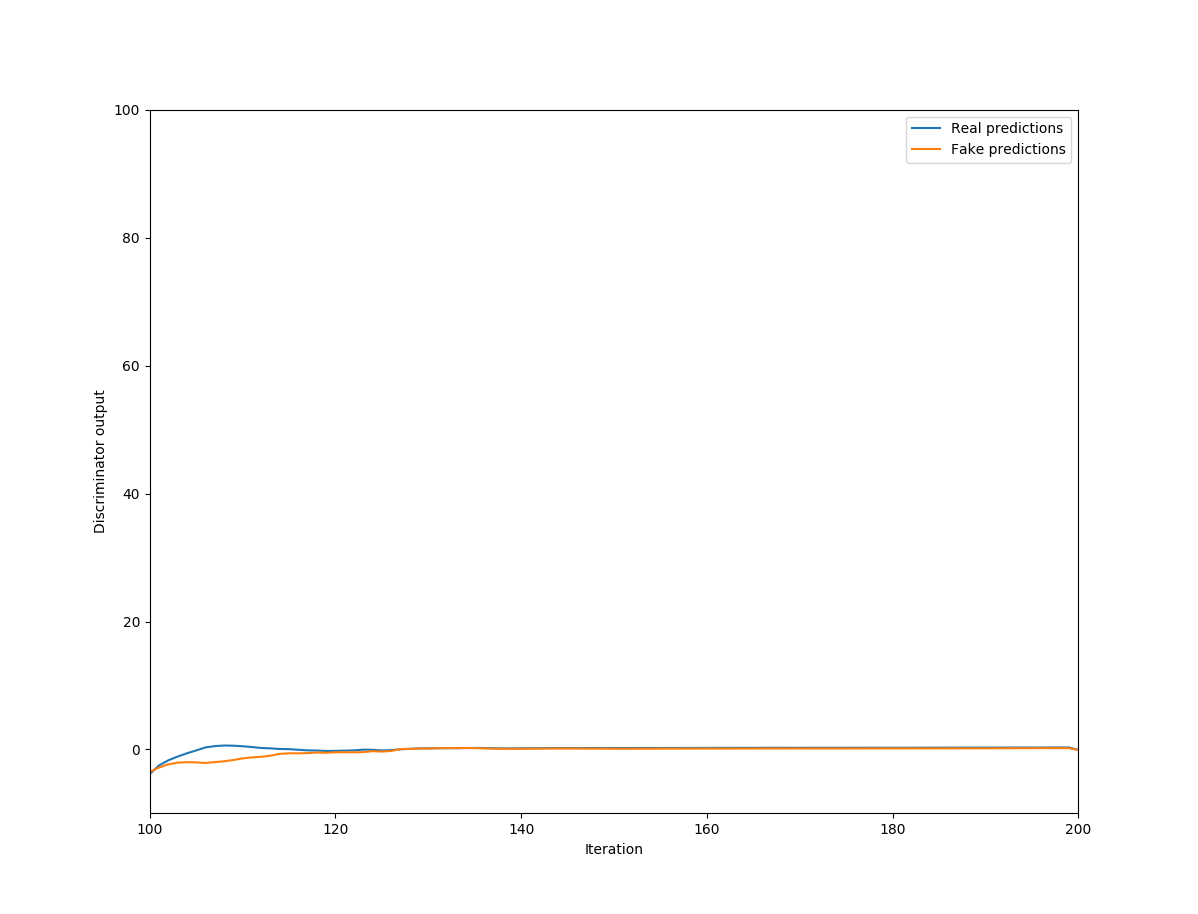
\includegraphics[width=\textwidth]{results/freezeInDG1.png}
%        \caption{Weight freezing in old layers}
%        \label{fig:freezeInDG1}
%    \end{subfigure}
%    \begin{subfigure}[b]{0.45\textwidth}
%        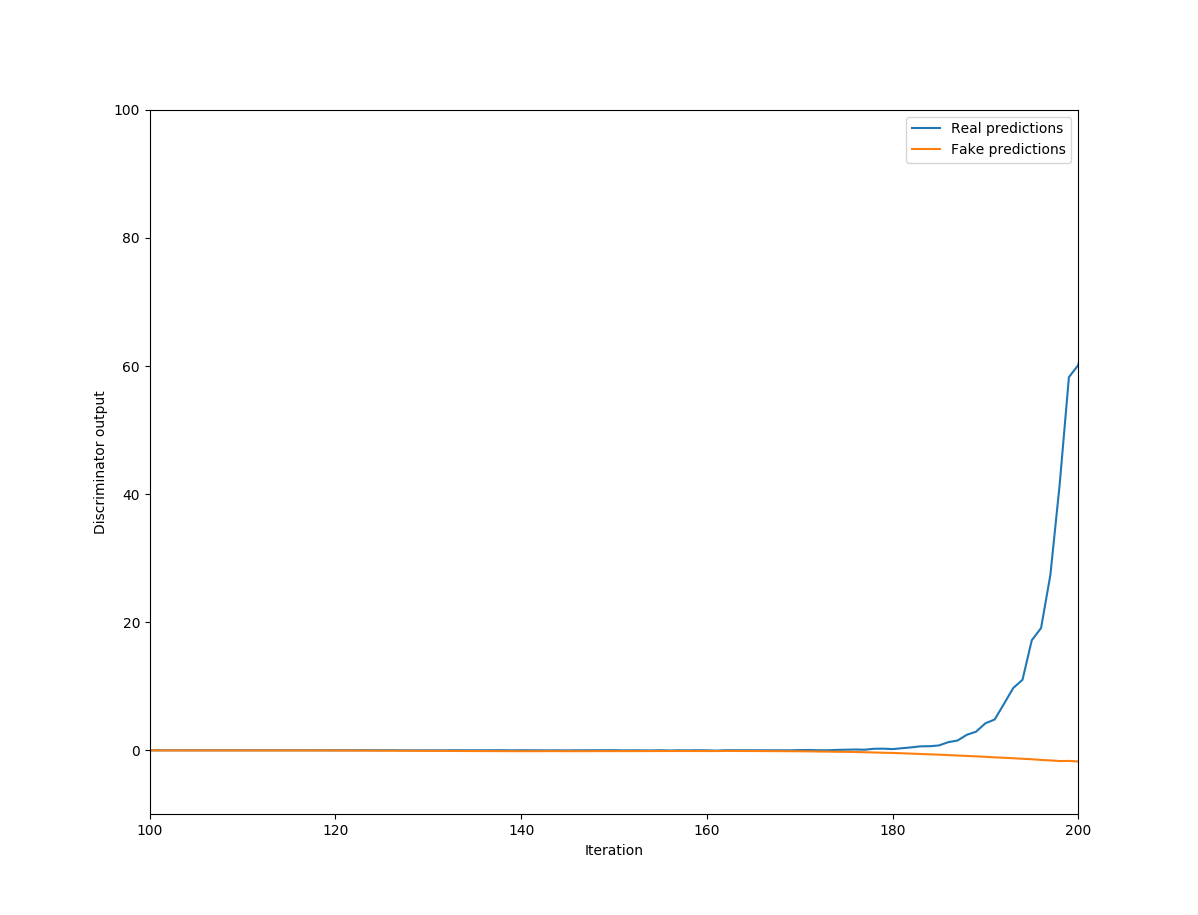
\includegraphics[width=\textwidth]{results/fadeInDG1.png}
%        \caption{Fade in new layers}
%        \label{fig:freezeInDG2}
%    \end{subfigure}
%    \caption{Discriminator output on real and fake images during transition between 16x16 and 32x32 resolution images for the different transition strategies.}
%    \label{fig:fadeVsFreeze}
%\end{figure}


\section{\acrlong{aegan}}
The final method tested in this project is based on a combination of autoencoders and \acrshort{gans}, named the \acrfull{aegan}. The proposed method consists of simultaneuously training a denoising autoencoder and a \acrshort{gan}, using the same network as generator and decoder. The idea is conceptually similar to the VAEGAN \todoproofread{add to acronyms} framework \parencite{LarsenSW15autoencodingbeyond}. There are two major differences between this method and the VAEGAN framework \st{, first} \todoproofread{. First} and foremost the autoencoder trained in this method is deterministic and trained with the mean squared error loss functions. Secondly, the adversarial loss is not used to train the autoencoder, instead a normal GAN is trained separately form the autoencoder but with the decoder network as the generator. 

Given enough capacity in the generator and encoder, the global minimum for the autoencoder training in this setting corresponds to the autoencoder learning the identity mapping. This causes the generator to generate realistic images on the points in the latent space the autoencoder maps the original data onto. The optimal generator in the \acrshort{gan} framework maps the entire latent space to realistic images. From this point of view the two objectives should lead to the same solution, however \acrshort{gans} tend to suffer from mode collapse and autoencoders often produce poor samples in terms of visual quality. Therefore if this method converges, it should enforce the decoded images to be sharp and the generator to capture the entire training data distribution. \todocomment{I think that this paragraph is a bit wordy and is hard to follow. You could maybe improve it by adding a diagram to help illustrate the relationships between the encoder, decoder and GAN with respect to the latent space as well as contrasting it with VAEGAN. It is also worth stressing that this is a unique contribution if you haven't already done so already.}
% Idé till presentationen: "Variational autoencoders are stable and good at ...blablabla... . On the other hand there are two major problems with variational autoencoders, 1: they are variational (Åtgärda KL-term), 2: they are autoencoders (pixel-loss ersätts med GANs)."

\section{Training setup}
For the experiments, all models were trained using the Adamax optimizer \parencite{kingma2014adam} with $8$ samples per batch, a learning rate of $0.0001$, $\beta_1 = 0.5$ and $\beta_2 = 0.99$. The non-progressive models were trained for around 440000 iterations, however convergence of the methods might be either much faster or much slower than this depending on the model. The progressive training consisted of $100000$ iterations per stage, with $10000$ iterations of fade in between the stages. \todocomment{Consider replacing $440000$ iterations with $440$k or $440,000$. It is easier to read.}


%Modelling annotated data: Normal GANs, image-to-image models.

%Modelling partially annotated data: Triple-GAN.

%Normalization technoques. Talk more about spectral normalization. 

%Implementation details: Highlight spectral normalziation observation (about weight matrix spectral norm in convolutional layer due to the shape). Talk about vectorization and viewing convolutions as a linear layer. 

\chapter{Results}
\begin{figure}[t]
    \centering
    \begin{subfigure}[b]{0.49\textwidth}
        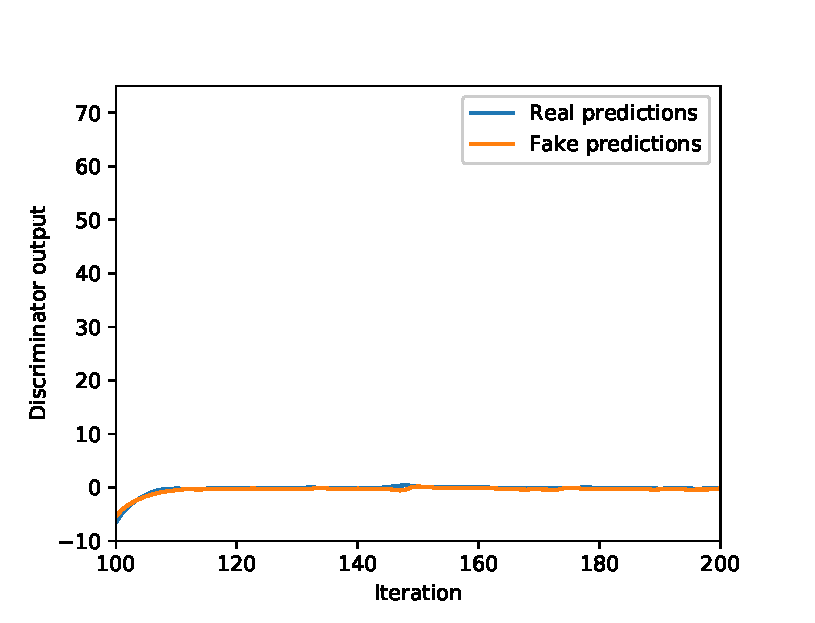
\includegraphics[width=\textwidth]{results/freezeInDG1_2.eps}
        \caption{Weight freezing in old layers}
        \label{fig:freezeInDG1}
    \end{subfigure}
    \begin{subfigure}[b]{0.49\textwidth}
        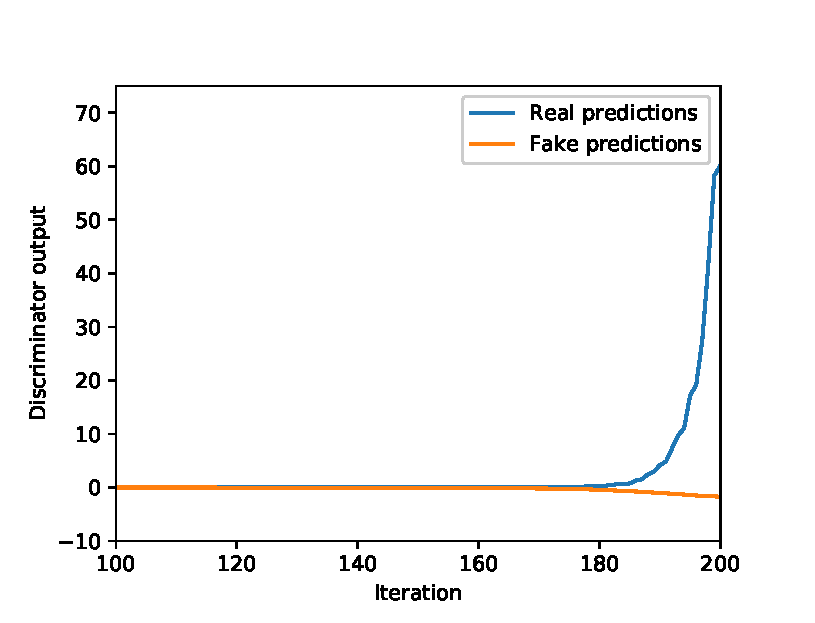
\includegraphics[width=\textwidth]{results/fadeInDG1_2.eps}
        \caption{Fade in new layers}
        \label{fig:freezeInDG2}
    \end{subfigure}
    \caption{Discriminator output on real and fake images during transition between 16x16 and 32x32 resolution images for the different transition strategies on the synthetic data set.}
    \label{fig:fadeVsFreeze}
\end{figure}

\begin{figure}[t]
    \centering
    \begin{subfigure}[b]{\textwidth}
        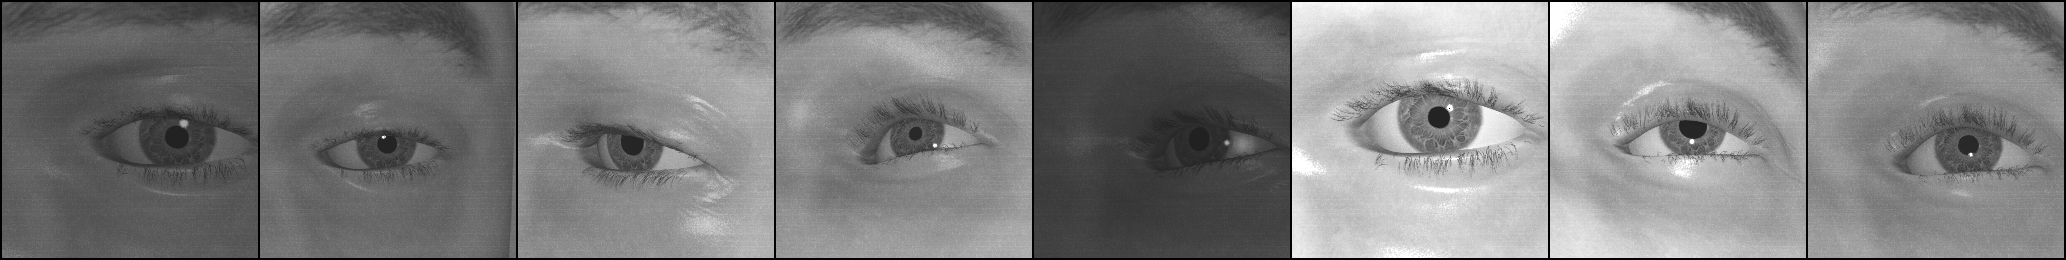
\includegraphics[width=\textwidth]{autoencoded/original.png}
        \caption{Original images}
        \label{fig:stuff}
    \end{subfigure}
    \begin{subfigure}[b]{\textwidth}
        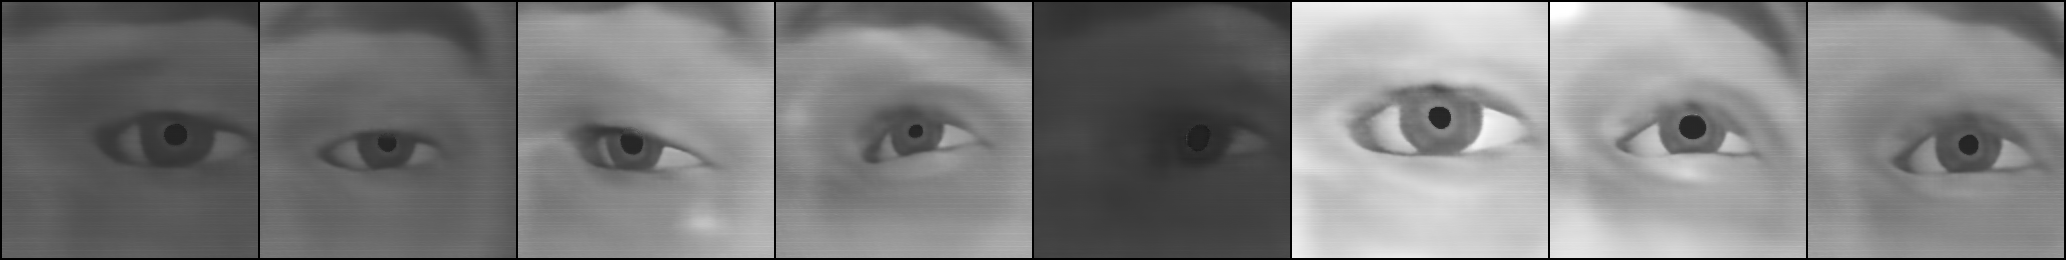
\includegraphics[width=\textwidth]{autoencoded/scaled_VAE_decoded.png}
        \caption{Decoded with VAE}
        \label{fig:stuff}
    \end{subfigure}
    \begin{subfigure}[b]{\textwidth}
        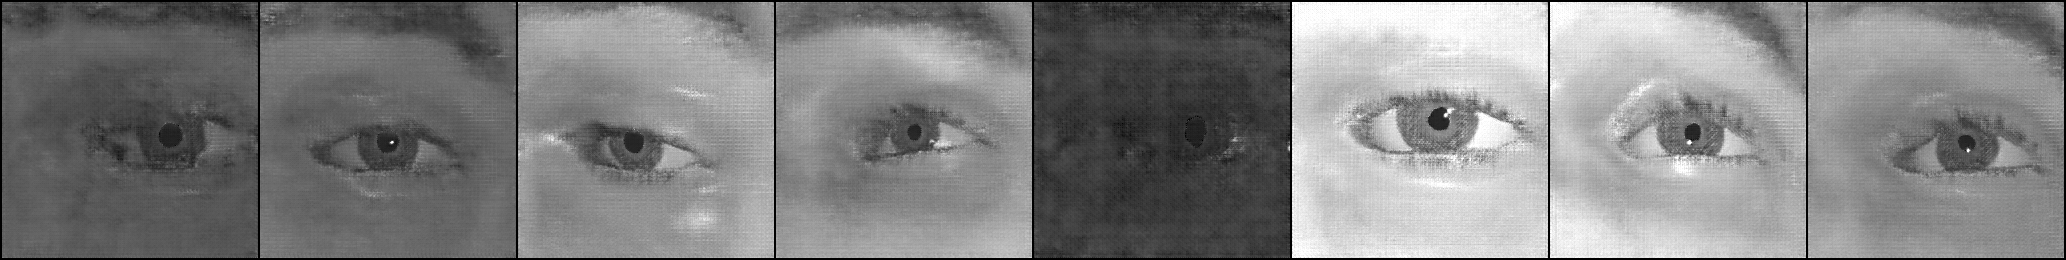
\includegraphics[width=\textwidth]{autoencoded/aegan_decoded.png}
        \caption{Decoded with \acrshort{aegan}}
        \label{fig:stuff}
    \end{subfigure}
    \caption{A batch of synthetic images, encoded and decoded by the encoder-decoder based methods.}
    \label{fig:autoencoders}
\end{figure}

\begin{figure}[t]
    \centering
    \begin{subfigure}[b]{\textwidth}
        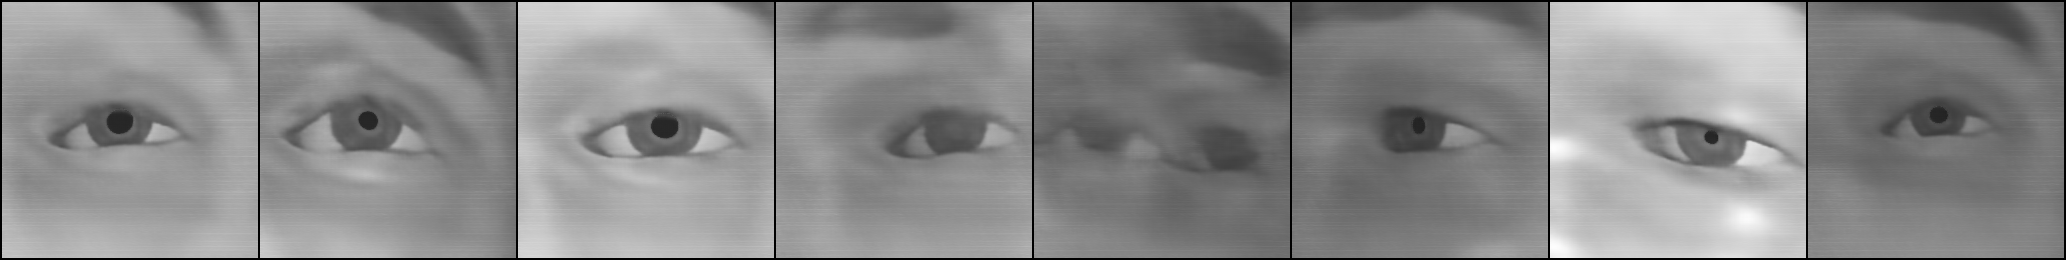
\includegraphics[width=\textwidth]{generated/vae_fake.png}
        \caption{Generated with VAE.}
        \label{fig:stuff}
    \end{subfigure}
    \begin{subfigure}[b]{\textwidth}
        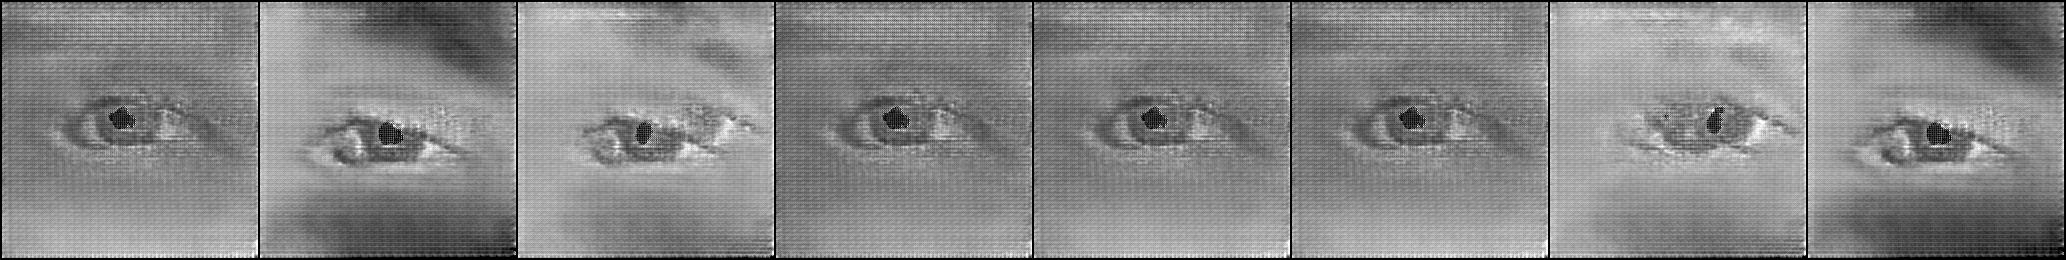
\includegraphics[width=\textwidth]{generated/wasserstein_fake.png}
        \caption{Generated with \acrshort{wgan}}
        \label{fig:stuff}
    \end{subfigure}
    \begin{subfigure}[b]{\textwidth}
        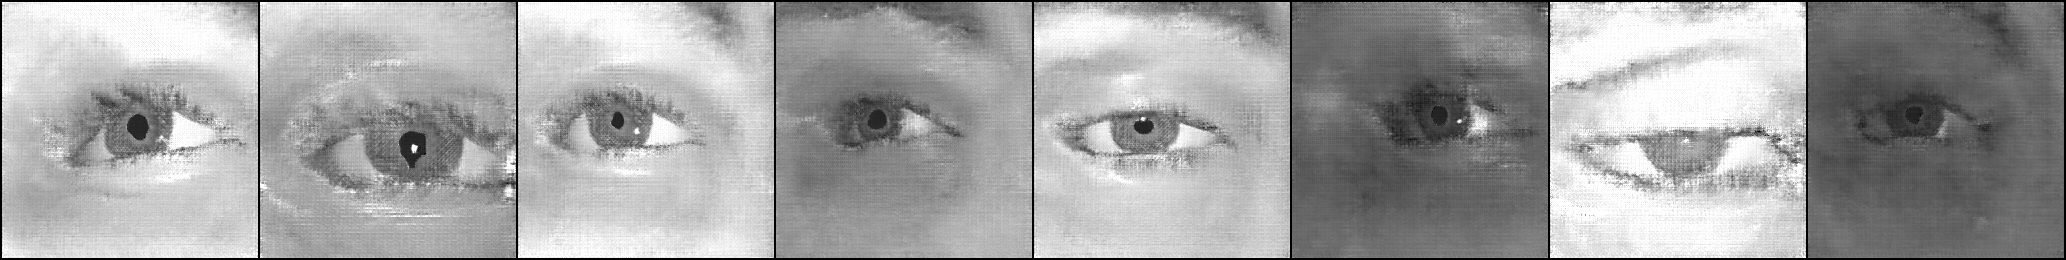
\includegraphics[width=\textwidth]{generated/aegan_fake.png}
        \caption{Generated with \acrshort{aegan}}
        \label{fig:stuff}
    \end{subfigure}
    \caption{Examples of a batch of generated images by the different models.}
    \label{fig:gans}
\end{figure}

\begin{table}[t]
    \centering
\caption{Jaccard distance between pupil regressor output and annotations for different sources of training data using synthesized data as the original data source. The leftmost columns indicate which data set the transformer was trained on. The test data used in \ref{subtab:on_real} is the original test set, whereas in \ref{subtab:on_fake} designated test sets were generated by the respective generative models.}
    \label{tab:quantitative_results}
    \begin{subtable}{0.9\textwidth}
        \begin{tabular}{|l|lll|}
            \cline{2-4}
            \multicolumn{1}{c|}{} & \multicolumn{3}{c|}{\textbf{Jaccard distance}} \\ \hline
            \textbf{Training data} & \acrshort{wgan} & VAE & \acrshort{aegan} \\ \hline
            Fake & \num{0.8132} & \num{0.159} & \textbf{\num{0.148}} \\
            Fake + real & \num{0.1219} & \textbf{\num{0.0944}} & \num{0.1032} \\
            \hline
            Real & \multicolumn{3}{c|}{\num{0.09607}} \\
            \hline
        \end{tabular}
        \caption{Tested on the real test data.}
        \label{subtab:on_real}
    \end{subtable}
    \begin{subtable}{0.9\textwidth}
        \begin{tabular}{|l|lll|}
            \cline{2-4}
            \multicolumn{1}{c|}{} & \multicolumn{3}{c|}{\textbf{Jaccard distance}} \\ \hline
            \textbf{Training data} & \acrshort{wgan} & VAE & \acrshort{aegan} \\ \hline
            Fake & \textbf{\num{4.82e-5}} & \num{0.0133} & \num{0.0491} \\ 
            Real & \num{0.1855} & \textbf{\num{0.0264}} & \num{0.1225} \\ 
            \hline
        \end{tabular}
        \caption{Test data generated by the generative models.}
        \label{subtab:on_fake}
        \end{subtable}
\end{table}

\begin{table}[t]
    \centering
    \caption{Jaccard distance between pupil regressor output and annotations for different sources of training data using models trained on real world data as original data. The structure and notation follows table \ref{tab:quantitative_results}.}
    \label{tab:quantitative_results_real}
    \begin{subtable}{0.9\textwidth}
        \begin{tabular}{|l|lll|}
            \cline{2-4}
            \multicolumn{1}{c|}{} & \multicolumn{3}{c|}{\textbf{Jaccard distance}} \\ \hline
            \textbf{Training data} & \acrshort{wgan} & VAE & \acrshort{aegan} \\ \hline
            Fake & \num{0.9966} & \num{0.3445} & \textbf{\num{0.2084}} \\
            Fake + real & \num{0.1215} & \textbf{\num{0.1151}} & \num{0.1221} \\
            \hline
            Real & \multicolumn{3}{c|}{\num{0.11456}} \\
            \hline
        \end{tabular}
        \caption{Tested on the real test data.}
    \end{subtable}
    \begin{subtable}{0.9\textwidth}
        \begin{tabular}{|l|lll|}
            \cline{2-4}
            \multicolumn{1}{c|}{} & \multicolumn{3}{c|}{\textbf{Jaccard distance}} \\ \hline
            \textbf{Training data} & \acrshort{wgan} & VAE & \acrshort{aegan} \\ \hline
            Fake & \textbf{\num{8.795e-6}} & \num{0.0284} & \num{0.0457} \\ 
            Real & \num{0.8798} & \num{0.1008} & \textbf{\num{0.0786}} \\ 
            \hline
        \end{tabular}
        \caption{Test data generated by the generative models.}
        \end{subtable}
\end{table}

\begin{table}[t]
    \centering
    \caption{Toy experiments on data augmentation}
    \label{tab:toy_experiments}
    \begin{subtable}{0.9\textwidth}
        \begin{tabular}{|l|ll|ll|ll|ll|}
            \cline{2-9}
            \multicolumn{1}{c|}{ } & \multicolumn{2}{c|}{Baseline} & \multicolumn{2}{c|}{WGAN} & \multicolumn{2}{c|}{VAE} & \multicolumn{2}{c|}{AEGAN} \\ \hline
            \textbf{Data set} & Mean & Std & Mean & Std & Mean & Std & Mean & Std \\ \hline
            Iris & \num{0.19751941} & \num{0.010727016} & \num{0.216506} & \num{0.0261355455} & \num{0.2040766} & \num{0.0093358} & \num{0.1780217} & \num{0.0084796728} \\
            \hline
        \end{tabular}
    \end{subtable}
    \begin{subtable}{0.9\textwidth}
        \begin{tabular}{|l|lll|l|l|}
            \cline{2-6}
            \multicolumn{1}{c|}{} & Baseline 100 & Baseline 200 & Baseline 400 & VAE & AEGAN \\ \hline
            Error rate ($\%$) & \num{0.90} & \num{1.02} & \num{0.87} & \num{1.33} & \textbf{\num{0.86}} \\ \hline
        \end{tabular}
    \end{subtable}
\end{table}


%\begin{table}[t]
%    \centering
%    \caption{Jaccard distance between pupil regressor output and annotations for different sources of training data using models trained on real world data as original data. The structure and notation follows table \ref{tab:quantitative_results}.}
%    \label{tab:quantitative_results_real}
%    \begin{tabular}{|ll|lll|lll|}
%        \cline{3-8}
%        \multicolumn{2}{c}{ } & \multicolumn{3}{|c|}{JD} & \multicolumn{3}{c|}{RD ($\%$)} \\ \hline
%        \textbf{Train} & \textbf{Test} & \acrshort{wgan} & VAE & \acrshort{aegan} & \acrshort{wgan} & VAE & \acrshort{aegan} \\ \hline
%        F & R & \num{0.9966} & \num{0.3445} & \textbf{\num{0.2084}} & \num{869.9} & \num{303.8} & \textbf{\num{183.8}} \\
%        F & F & \textbf{\num{8.795e-6}} & \num{0.0284} & \num{0.0457} & \textbf{\num{0.00768}} & \num{25.0} & \num{40.3} \\ 
%        R & F & \num{0.8798} & \num{0.1008} & \textbf{\num{0.0786}} & \num{768.0} & \num{88.9} & \textbf{\num{62.3}} \\ 
%        F + R & R & \num{0.1215} & \textbf{\num{0.1151}} & \num{0.1221} & \num{106.1} & \textbf{\num{101.5}} & \num{107.7} \\ 
%        \hline
%        R & R & \multicolumn{3}{c|}{\num{0.11456}} & \multicolumn{3}{c|}{100} \\
%        \hline
%    \end{tabular}
%\end{table}

%\begin{table}[t]
%    \centering
%    \caption{Jaccard distance between pupil regressor output and annotations on synthetic data}
%    \label{tab:quantitative_results}
%    \begin{tabular}{l|l|l}
%    \hline
%    %\multicolumn{3}{c}{Generator}           \\ 
%    Training data type      & MEE synthetic data  & MEE Accuracy real data \\ \hline
%    Original data           & $\sim$ 0.3 & 1.1     \\
%    VAE                     & $\sim$ 1.7 & 1.9     \\
%    VAE + original data     & 0.3 (guess) & 134     \\
%    %PGAN                    & 5.4 (pessimistic guess) & 134     \\
%    %PGAN + original data    & 0.3 (optimistic guess) & 134     \\
%    \acrshort{aegan}                   & 0.3 (optimistic guess) & 134     \\
%    \acrshort{aegan} + original data   & 0.3 (guess) & 134     \\
%    \end{tabular}
%\end{table}

A set of exploratory experiments were conducted for the different proposed methods to find settings where the methods succeed at producing visually pleasing data. Due to the unstable nature of \acrshort{gans} and the limited available resources in this project, most of experiments based on \acrshort{gans} failed to do this. The few successful models also turned out to be highly sensitive to changes in network architecture, hyperparameters or training setup leaving a loot of room for improvement and further investigations. 

Of the tested methods, only the \acrshort{vae} and \acrshort{aegan} were capable of producing data with some visual resemblance to the original data. The Wasserstein GAN suffered from severe mode collapse and training instability thereby resulting in only failures.

The progressive \acrshort{gan} produced promising results on the initial stages with highly downsampled data. However the proposed fade-in procedure failed, forcing the model to re-learn everything from scratch at each stage of training. At the lower stages the model was capable of recovering after the fade-in but not on the full resolution stage, resulting in behaviour similar to the normal \acrshort{wgan}. 

To circumvent the fade-in issues of the progressive \acrshort{gan} an alternative freeze-in method of introducing the layers was tested. This approach views the introduction of the new layers as a transfer learning problem and freezes all but the newly introduced weights for a number of iterations. The method resembles gradual tuning for transfer learning \parencite{montone2017gradual}. The discriminator output of the progressive \acrshort{gan} during fade-in and freeze-in is illustrated in figure \ref{fig:fadeVsFreeze}. In this figure one can see that the freeze-in strategy results in a more stable transition between the stages. However this strategy requires the adversarial game between the last layers of the generator and the first layers of the discriminator to be balanced for all transitions which was observed not to be the case, which is why the progressive \acrshort{gan} is not featured in any further evaluation.

\section{Qualitative Results}
Figure \ref{fig:autoencoders} shows a batch of images, together with the same batch after being encoded and decoded by both a \acrshort{vae} and an \acrshort{aegan}. From this figure it is clear that both of these methods have managed to learn to capture the main aspects of the full data distribution. Both methods display varying illuminance levels, pupil dilations, different reflections and eyelid openness. However it is common for both methods to fail to capture the original information in some of these such as pupil dilation. Even though the methods display a clear variance in pupil dilation, the reconstructed dilation does not always correspond to the original pupil size.

The single most striking observation to emerge from comparing these images is the level of details captured by the \acrshort{aegan}. Unlike the \acrshort{vae}, the \acrshort{aegan} learned to produce glints and sharp eyelashes. It is also interesting to note that the glints are sometimes correctly positioned which due to the structure of deep convolutional neural networs is not easily learned. However in many cases it can be seen that the glints are poorly placed.

Decoding images from a learned posterior is not the same as generating new images from the prior distribution. Examples of generated images from a $\mathcal{N}(0, 1)$ distribution are shown in figure \ref{fig:gans}. In this case the \acrshort{wgan} is also featured as it allows sampling new data. 

What stands out in this figure after observing the decoded images is the \acrshort{vae} images, which sometimes looks decent as before but in some cases looks more artistic than realistic. Except for this observation, it is also clear from the figure that the \acrshort{wgan} suffered from severe mode collapse wereas the \acrshort{aegan} managed to capture both a good variance and visually pleasing quality of some of the samples even though some artefacts easily can be spotted in most images.

% However, failing to position the glints correctly causes the \acrshort{gan} objective and the autoencoder loss to operate in different directions, as the autoencoder loss will penalize the existance of wrongly placed glints causing the model to generate more modest and non-realistic glints which in turn will be penalized by the \acrshort{gan}.  <- Diskussionsmaterial ? 

% ...
%A comparison between a VAE and the autoencoder part of an \acrshort{aegan} is shown in figure <Referera till figur>. It is clear from this illustration that the simultaneous training of the GAN caused the autoencoder to generate more visually pleasing samples.

\section{Quantitative Results}
For the quantitative evaluation the default transofrmer was trained to generate segmentation maps from images of eyes. The images in this context can be directly from one of the data sets as well as from a generative model trained on one of these data sets. In the first case the images are denoted as "real" images, and in the second case they are denoted as "fake". 

The difference between the predicted segmentation map and the original was defined as the Jaccard Distance, defined as
\begin{equation}
    D_{Jaccard}(X, Y) = 1 - \frac{X \cap Y}{X \cup Y},
    \label{eq:jaccard}
\end{equation}
where the sets $X$ and $Y$ is the set of activated pixles in the respective segmentation map, which corresponds to the set of $1$:s for the real annotations. Any segmentation map generated by a neural network may include any floating point value for each pixel. These values were therefore rounded to produce a binary segmentation map. In this evaluation there exists images without pupils in some images, this results in computing the Jaccard distance between the empty set. To solve this all sets implicitly contain an extra element common to all sets. This can easily be computed as it only requires adding $1$ to the denominator and numerator in the fraction in (\ref{eq:jaccard}).

The Jaccard distances for segmentation maps produced by transformers trained and tested on different data sets is shown in table \ref{tab:quantitative_results} for the models trained on synthetic data and in table \ref{tab:quantitative_results_real} for the models trained on the real world data. The most important results in both of these tables is the first row which roughly corresponds to the direct usability of the generated data. In both cases, the \acrshort{aegan} performed best for this measure indicating as already qualitatively observed that the \acrshort{aegan} produced the best data sets. Another interesting finding is that training on both generated data and real world data did not increase the perfromance on real data for any of the cases except the \acrshort{vae} on synthetic data, where the test distance were slightly lower thant the original test distance.

%\section{The effect of sampling bias}  % - borde skriva om detta i metod-delen också
%TODO: Undersök om AEGANv2 kan augmentera MNIST med förbättrat resultat. Kontrastera resultat mot v1 med tolkningen att v2 är mindre påverkad av sampling-bias. Samma sak bör göras med VAE. Ifall posterior-augmentering är bättre än vanlig så bör uppskalade experiment också genomföras.

\section{Augmenting data for classification}
% TODO: Formulera om Iris som klassificeringsprblem

In the case of discrete classification there is no obvious method for concatenating data with the annotations. On the other hand it is sensible to assume that a small peturbation of an image does not alter the class label. With this assumption the autoencoder-based methods can still be used for data augmentation. Instead of sampling the latent points for the new data from the prior distribution $P(Z)$, they are sampled from the posterior $P(Z|X=x)$ yielding new data points. This procedure was tested on the MNIST dataset, the results are illustrated in table \ref{tab:toy_experiments}.

%In table \ref{tab:quantitative_results}

%Quantitative results can be seen in table \ref{tab:quantitative_results}.



%\begin{table}[t]
%    \centering
%    \caption{Number of iterations of training for the different algorithms}
%    \label{tab:quantitative_results}
%    \begin{tabular}{l|l|l}
%    \hline
%    %\multicolumn{3}{c}{Generator}           \\ 
%    Training data type      & Synthetic data  & Real data \\ \hline
%    VAE                     & 560000 & 560000 \\
%    PGAN                    & idk & idk     \\
%    \acrshort{aegan}                   & 520000 & 840000   \\
%    \end{tabular}
%\end{table}

%TODO: Visa kapacitet/overfitting på samma dataset, visa att genererad data är konsistent och har bra annoteringar!

%<<Lägg till ett par histogram här.>>

%<<Figur med referensbatch och decoded för VAE, AE och \acrshort{aegan}. Inkludera L1-fel för samtliga rekonstruktioner>>




\chapter{Discussion}
% Stycke om progressive GAN och varför jag tror fade-in inte funkar för binär data
This study set out with the aim of assessing the posiblitities of using deep generative models for data augmentation when training deep neural networks on complex data sets. The results of the study confirms that \acrshort{gans} are associated with a highly unstable training procedure, whereas \acrshort{vaes} are more stable and capable of producing more predictable image reconstructions. The most important finding was that \acrshort{gans} can be improved by simultaneous training of an autoencoder. Unlike previous methods combining \acrshort{gans} and autoencoders \parencite{LarsenSW15autoencodingbeyond, nguyen2016plug, donahue2016adversarial, ulyanovVL17adversarial}, no explicit coupling between the autoencoder and \acrshort{gan} exists. Insted sharing generator parameters and the latent space was shown to be sufficient for generating better data sets than any of the baseline methods.

One unanticipated finding in this project was that the fade in approach of \textcite{karras2017progressive} failed to preserve the learned information between the stages of the progressive \acrshort{gan}. A possible explanation of this is that the generator learns to mute the residual connection and compensate by scaling the original signal during the majority of the fade in period. When the fade-in almost is finished and the signal moves towards only using the new connections, the new parameters remains untrained rendering the whole process useless. The fact that this behavior is not reported in \parencite{karras2017progressive} suggests that it is data-dependent. Since the segmentation maps are binary, fake maps can easily be distinguished if they are scaled which indicate that this phenomenon might be triggered by this property of the data. However further investigations are necessary before this can be stated for certain.

The problem of mode collapse is one of the main research frontiers of \acrshort{gans}. The extremely low fake-fake score for the \acrlong{wgan} suggests this model suffered from severe mode collapse. By inspecting the generated images it is clear that this is the case. This outcome is contrary to the original claim by \textcite{arjovsky2017wasserstein} that these models should be liberated from mode collapse. However to be fair, this claim assumes the discriminator to be trained to optimality between each generator iteration which in practice is infeasible. 

Wile the \acrshort{wgan} suffered from severe mode collapse, both the \acrshort{vae} and the \acrshort{aegan} seem to have learned to capture most of the variance in the original distribution. For the \acrshort{vae} this result is quite expected as mode collapse generally is not a problem for these models. Furthermore, since it moslty learns low-frequency features of the data, there is less variation left to be learned making the accomplishment less impressive. The \acrshort{aegan} on the other hand is partially a normal \acrshort{gan} and should be very susceptible to mode collapse. The fact that it manages to capture the levels of variation in pose, illuminance, eyelid openness etc. suggests that the simultaneous training of an autoencoder improved the the variation of the generated samples as proposed.


%It is believed that this mode of failure is data dependent. Further research on MNIST is proposed to asses this case.

%Diskutera mode collapse. Förvånansvärt litet problem i både AEGAN och karras (tror jag). Kanske minibatch-std som gör det. Sannolikt att AEGAN-ramverket hjälper också, men kan nog inte påstå det.

% TODO: Diskutera metoder som inte hann testas, svårt att säga att AEGAN är bäst.

The present study was as stated designed to determine the effect of training neural networks on data generated by deep generative models. It is reasonable to believe that generated datasets that are qualitatively similar to the original data in terms of visual quality and variation results in better neural networks when training on the generated data. The results of this study indicate that this is the case. 

It is somewhat surprising how well the numbers of the first row in the first subtable in the tables \ref{tab:quantitative_results} and \ref{tab:quantitative_results_real} correspond to the previously discussed visual quality of the data sets. 
The high Jaccard distance for the \acrshort{wgan} can be explained by the severe mode collapse that the model suffered from, making it very difficult to learn anything usable from this model for the semantic segmentation network. Moreover the loss of high-frequency details in the \acrshort{vae} seem to have had a similar effect, making it more difficult to generalize to the real data given only this data. However in this case the generated data seem to be somewhat usable, giving quite reasonable jaccard distances. The \acrshort{aegan} produced both a good variance and decent looking images with high-frequency details, even though they contained some artifacts and could without too much effort be distinguished from the real data. This resulted in the best jaccard distances when training solely on the generated data in both cases.

Considering the data augmentation test in the first subtable of tables \ref{tab:quantitative_results} and \ref{tab:quantitative_results_real} instead of the stand alone case for the generative models, it can be observed that the best stand-alone generative model is not the same as the best generative model for data augmentation. Instead the \acrshort{vae} resulted in the lowest Jaccard distance for both the synthetic data and the real world data sets. It seems possible that these results are due to the artifacts produced by the \acrshort{gan} training. When observing the results from training on real data and testing on synthetic one can see that the only case where the jaccard distance is lower than the baseline is when tested on the \acrshort{vae} images. An interpretation of this is that the absence of high-frequency details causes this data to be easier than the original data in terms of predicting the pupil positions. This means that introducing these images during the training process of a normal network gives relatively small gradients and does not introduce false patterns that the learning process may adjust to. In other words, the \acrshort{vae} does not cause as much harm to the training as the other models may do. 

On the other hand, using the same argument it is sensible to suspect that the \acrshort{vae} is unlikely to provide the type of data that a network could benefit from during training in settings where the need for data augmentation is higher than the pupil regression experiments where the existing data volume is more than sufficient for the purpose. This suspicion is further confirmed by the toy experiments presented in table \ref{tab:toy_experiments}

% TODO Ge wgan lite cred ändå och säg att den hade kunnat få en bättre chans


\chapter{Conclusion}
This study has shown that deep generative models can be applied to generate synthetic data sets that can be used to boost the performance of existing discriminative models. The experiments revealed some settings where this likely is the case. It was also illustrated that with a simple task and a large data set, a discriminative model can be used to evaluate the quality of the generated data sets. Although this study focuses on data augmentation, this finding may well have a bearing on how to benchmark different \acrshort{gans} in general. 

The scope of this study was limited in terms of time and computational resources, and therefore several questions still remain to be answered. Notwithstanding these limitations, this study strenghtens the idea that synthetic data sets can be used as drop-in replacements for existing data sets and it lays the groundwork for future research into generating usable data with deep generative models.

\section{Future work}
TODO: Write stuff here if I want to.


% --------------------------------------------------------------------------------------------------------

\printbibliography[heading=bibintoc] % Print the bibliography (and make it appear in the table of contents)

\appendix

\chapter{Lots of images here}

\end{document}
